\documentclass[12pt]{article}
\usepackage[margin=3cm]{geometry}
\usepackage{blindtext}
\usepackage{chngcntr}
\counterwithin*{section}{part}
\usepackage{enumitem}
\usepackage{listings}
\usepackage{float}
\usepackage{graphicx}
\usepackage{tikz}
\usepackage{subfig}
\usepackage{hyperref}
\usepackage{amsmath}
\usepackage{multicol}
\usepackage{tcolorbox}
\usepackage{xcolor}
\lstset{language=C++,
    basicstyle=\ttfamily,
    keywordstyle=\color{blue},
    stringstyle=\color{red},
    commentstyle=\color{green},
    morecomment=[l][\color{magenta}]{\#}
}

\hypersetup{
    colorlinks=true,
    linkcolor=blue,
    citecolor=green,
    urlcolor=red
}
\usetikzlibrary{quotes, angles, decorations.markings, intersections}
\usetikzlibrary{calc,patterns,angles,quotes, 3d, intersections, positioning, shapes, automata, positioning}
\newcommand{\tbox}[1]{\noindent\fbox{\parbox{\textwidth}{#1}}}
\title{OS CS219 Notes}
\author{}
\date{\today}
\begin{document}
\maketitle
\setlength{\parskip}{6pt}
\setlength{\parindent}{0pt}

\noindent\tbox{
    \begin{center}
    \textbf{\Huge Lecture 1}
    \end{center}
}
\part{Introduction to Operating Systems}
\section{Introduction}
\noindent An \textbf{OS}(operating system) alias \textbf{Master Control Program} alias \textbf{System software} is software than enables the user to access the hardware resources of a computer 
in a controlled manner. It acts as a layer of abstraction allowing the user to not worry
about hardware level access and just provides access to a few methods needed by the user


\noindent The OS has several uses/functions in a computer
\begin{itemize}[topsep=0pt, partopsep=0pt, itemsep=0pt, parsep=0pt]
    \item Manages resources as a single \textbf{central entity} and hence efficiently
    \item \textbf{Virtualizes} physical resources to be utilized by multiple processes\footnote{process is defined later}
    \item \textbf{Isolates} and protects processes from one another by not allowing direct access to hardware 
    \item Provides a set of system calls for the user to access hardware resources
    \item Starts processes and allocates and manages memory required by said process during execution
\end{itemize}

\noindent Thus it is easy to see that the OS has several important functions to perform inorder to enable an abstraction of hardware from the users

\section{Process and Virtualization}

\noindent A process is just the sequence of execution of instructions by the CPU
. When we write and compile a program it gets converted into a sequence of instructions whose first \textit{instruction address} is fed to the PC and as we know 
the sequence of instructions for that program starts getting executed one by one. This is called a process. So when we run a program a \textit{process} is created.


\subsection{Context switching}
\label{section:context}
How do we tell the CPU to start a process. First obviously we need to feed the address of the first instruction of the process to the \textbf{Program Counter}. We also need to set 
the stack pointer and other registers with appropriate values. This is called \textbf{setting up the context} for a process. This job is done by the OS. After the context is set the OS takes a back seat and allows the CPU to do its work


\noindent However this has a few issues. Firstly, when the process requests for data from say the hard drive there is a gap where the CPU 
is on standby which is wasteful since other processes also require it. Secondly, we also want responsiveness from our system (ie) when
we have a process running we also may want to interact with other processes. 


Both of these issues are solved by \textbf{concurrent} execution. Basically we run a process for a while and when the CPU is on standby or after a 
particular interval of time we save the \textit{context} (ie) states of all registers including PC and start the other process by setting up its context this repeats
for a while and eventually the partially executed process's context is set and it is continued.
This is reffered to as \textbf{context switching} and is an important part of Virtualization\footnote{Read further to know what it is} of the CPU.
Note that a part of the OS (ie) \textit{OS scheduler} decides which program to run at what time

\subsection{Virtualization}
Virtualization refers to the creation of an illusion that each of the processes have full access hardware resources\footnote{It is useful to think of Virtualization as the OS lying to each process about it having full access to a resource}. This
enables the hardware to act much more powerfully than they are capable of. For example, as mentioned above context switching creates the illusion
of the presence of multiple cores each assigned to one process whereas in reality it is just one core.
Infact this is refered to as \textbf{Hyperthreading}. Apart from the CPU memory, addresses can be virtualized.

\section{Memory allocation and Isolation}
\label{section:mem_alloc}
\subsection{Memory}
As we learnt in CS230, memory for a process/program is allocated as a fixed number of bytes. The inital bytes
of this memory is the instructions and the global/static variables. Local variables aren't initialised in memory since
we do not know the number of times each function is called, instead we have a dynamically growing stack whose starting address is
stored in the special \textit{stack pointer register}. This stack grows and shrinks as necessary functions are called and they return values.
\footnote{The structure used here is a stack since functions are inherently \textit{LIFO} functions called last return first}.


Apart from this we have a heap which can be accessed by user to store dynamically increasing data structures. We can request the
OS to allocate certain number of bytes and return a pointer to said bytes


Here again however the OS plays tricks on the processes. Since it is impractical for the OS to allocate to 
allocate memory for the process continguosly it allocates them in chunks but returns a \textbf{virtual address} (Recall Virtualization) to the program. This "virtual address" is the
address returned when the user requests the OS for an address of the data stored. Here again the OS lies to the process creating the illusion that it has access to continguos memory starting
from some location
\newpage
\noindent\tbox{
    \begin{center}
    \textbf{\Huge Lecture 2}
    \end{center}
}
\subsection{Isolation}
    \label{section:Isolation}
    Now we understand that the OS allows multiple processes to run at the same time and share resources
    But this raises a huge issue since processes are supposed to be independent and processes being to affect other 
    processes would cause problems. The OS takes care of this too by maintaing strict control over access to hardware

    The OS is the only entity with access to hardware and process can make specific requests to the OS to use hardware
    via \textit{system calls}\footnote{syscalls can't be accessed directly usually. They are in a language's standard library}. Infact there are two types of instructions and processer modes corresponding to them

    \begin{itemize}[topsep=0pt, partopsep=0pt, itemsep=0pt, parsep=0pt]
        \item \textbf{Privileged instructions} - special instructions that can interact with hardware. Generated by syscalls,device drivers
        CPU is in \textbf{kernel} mode while executing them 
        \item \textbf{Unprivileged instructions} - simple instructions that do not need access to hardware. Given by user processes. CPU is in \textbf{user} mode while running them
    \end{itemize}

    The CPU is always in user mode except the following cases.
    \begin{itemize}[topsep=0pt, partopsep=0pt, itemsep=0pt, parsep=0pt]
        \item A syscall is made
        \item Interrupt occurs
        \item Error needs to be handled 
        \item Context switching needs to happen for say concurrent running
    \end{itemize}
    
    Note that when a syscall is made the OS code pertaining to it is executed and then control is return back to user code
    \\\textbf{Interrupt:} In addition to running programs a CPU has to handle external inputs from devices like a mouse click.
    This is called an Interrupt. During an interrupt control is given to the OS(Kernel mode of CPU) which deals with the interrupt and returns
    control to the user process \footnote{This means saving context, handling the interrupt and setting context of the past status}


    \noindent\textbf{Device Driver:} I/O is managed by the device controller(Hardware) and device driver\\(software)\footnote{This is part of the OS}.
    The driver initializes IO devices and it starts IO operations like reading from the disk. It also handles the above mentioned interrupts


    \section{Process abstraction and attributes}

    As we have discussed above about a process it is a sequence of instructions running in the cpu.
    Also as discussed in section \ref{section:context} a process can run for a while, then be blocked and run again.
    Hence a process switches from one \textit{state} to another during its execution. We can note that this process state changes only when the kernel goes to user mode.\footnote{Since the change is done by the kernel's OS scheduler}

    \begin{figure}[h]
        \centering
        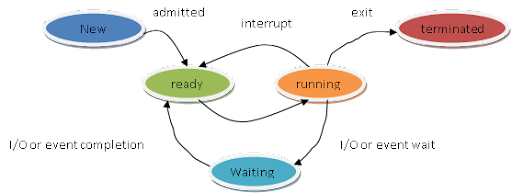
\includegraphics[width = 10cm]{process-state.png}
        \caption{Figure to show process state switching}
        \label{process-state}
    \end{figure}
    {\large A process is defined by several \textit{attributes} that define it:}
    \begin{itemize}[topsep=0pt, partopsep=0pt, itemsep=0pt, parsep=0pt]
        \item \textbf{PID}: Unique process identifier given to each process
        \item \textbf{PPID}: PID of a parent process\footnote{Parent discussed later}
        \item \textbf{Context}: Context is saved when switching happens. We have discussed what the context of a process refer \ref{section:context}
        \item \textbf{File descriptors}: A record of all the files open by a process is stored in form of pointers in 
        an array. Elements at index 0,1,2 refer to std input, std output and error files. As we open more files for
        a process a pointer to it is created and added to the end of the array. This poiner is what is returned as a 
        \textit{file descriptor} for the user to perform read or write operations.
        \item \textbf{State}: A process can be in 3 states
        \begin{enumerate}[topsep=0pt, partopsep=0pt, itemsep=0pt, parsep=0pt]
            \item \textbf{Running}: The CPU is currently executing instructions of the process
            \item \textbf{Blocked/suspended}: The process cannot run for a while. Maybe it requested data from drive and is waiting for its arrival
            \item \textbf{Ready/runnable}: Process can be run and is waiting for \textit{OS scheduler} to give it a CPU/core to use
        \end{enumerate}
        \item \textbf{Memory}: Each process uses/is allocated a fixed amount of memory by the OS and its locations are stored
        \item \textbf{Page Table}: The OS lies to the process about memory addresses(Virtual address \footnote{refer Section \ref{section:mem_alloc}}). The real address mapping to the corresponding
        virtual address is stored in the page table. The page table can be used to get the real address corresponding to each virtual address
        \item \textbf{Kernel Stack}: The context of a CPU is saved in this kernel stack when context switches occur. This stack is stored in a seperate memory and it isn't accesible by user code
        The OS uses this stack since it doesn't trust the user stack. Each process has its own kernel stack
    \end{itemize}


    \subsection{Process Control Block}
    All the above mentioned attributes of a process along with more necessary information
    is stored in a data structure called the process control block(PCB)\footnote{Stores the details about one process}


    It is called by different names in different OSes:
    \begin{itemize}[topsep=0pt, partopsep=0pt, itemsep=0pt, parsep=0pt]
        \item \textit{struct\_proc} in xv6
        \item \textit{task\_struct} in linux
    \end{itemize}


    The above mentioned attributes of various processes are stored in the PCB 
    in form of the \textbf{ptable} or process table which is a data structure storing all the 
    \textit{proc structs} each of which has all the data corresponding to each process

    In \textbf{xv6} the ptable is just an fixed size array since it is a simple system. However in real
    world kernels it is a dynamically expanding data structure. 

    
    The \textbf{OS scheduler} iterates over the ptable picks a \textit{ready} process and assigns it a processor to run it.
    A process which needs to be put to sleep (Eg. IO from disk) will be put to sleep and another is picked from processor
 
    \section{Booting}
    We need some system to load up our OS into the CPU during start of the system.
    The \textbf{BIOS}(Basic input output system) is present in the non-volatile memory of our system which locates boot loader 
    in the boot disk. It is a simple program whose job is to locate and load the OS. It is present in the first sector of the boot disk
    It sets up context for the kernel and gives control to kernel


    \textbf{BootLoader} must fit in 512 bytes of the Boot disk to be easily located which isn't sufficient to load up current complicated systems.
    So the 512 bytes(simple bootloader) load up a more complex BootLoader which loads OS onto the CPU 
\newpage
\noindent\tbox{
    \begin{center}
    \textbf{\Huge Lecture 3}
    \end{center}
}

\part{Process Management}
\section{API:Application Programming Interface}
\textit{System calls} provide an interface to the OS called the Application Programming Interface (ie) the set of syscalls given
to the user constitute the \textbf{API},

Two types of syscalls are:
\begin{itemize}[topsep=0pt, partopsep=0pt, itemsep=0pt, parsep=0pt]
    \item \textbf{Blocking:} Syscalls that block the process that called it\footnote{Like when you wanna read from disk which takes time} and the OS comes back to the user process after a while
    \item \textbf{Non Blocking:} Syscalls that are called with the user instructions which acts along with user process without blocking the calling process\footnote{The process which calls the syscall} since they return immediately (eg. getpid())
\end{itemize}


If every OS has different syscalls \textit{portability}\footnote{ability to run same code on multiple machines} is an issue. For this purpose all the OS providers decide on an universal set of syscalls
\footnote{The implementation of said syscall may differ} to provide called the \textbf{POSIX} API. Interestingly, since the instructions for syscalls maybe different this is why we may have to recompile to run code on another OS

Hence the hierarchy of a syscall is somewhat like:
\begin{center}
    User code $\rightarrow$ Standard library functions $\rightarrow$ Syscall in the function $\rightarrow$ Syscall in assembly instruction $\rightarrow$ OS
\end{center}

In xv6 we are directly given syscalls in the standard library in a user friendly function call. Usually we are given syscalls at the assembly code level
since we usually need to change the privilege of CPU\footnote{Done using INT in assembly}. Hence we need to understand that syscall is \textbf{NOT} a regular function call.\footnote{Lottt more detail on this further}

\subsection{Fork}
Each process is created by another process. Such a process emerging from another is called the \textit{child} of the \textit{parent} process.
The syscall used to create such a process is called \textit{fork}. \texttt{Init} is the initial process from which all other processes are \textit{forked}.

When you call fork:
\begin{itemize}[topsep=0pt, partopsep=0pt, itemsep=0pt, parsep=0pt]
    \item New child process is created with new \textbf{PID}
    \item Memory image\footnote{the heap,stack,instructions,data is the memory image of a process} of the parent is given to the child
    \item They run copies of same code
\end{itemize}
Note that while the child may share the virtual memory with parent. It is in a different physical memory location


What is the point of running the same process as a child again? There is none. They aren't the same process due to one key difference.
The \texttt{fork()} returns 0 in the child process and returns the PID of child to the parent. Hence we can make the parent and child run different code
using the different value returned by the \texttt{fork()} function. Note that \texttt{fork()} returns -1 when forking fails. This process seems to be generating different process running some redundant code.
This is not the way to create process to perform very different functions as compared to parent.
We will see another way to create processes for that case
later. Interestingly as of yet the parent also needn't run before the child since they are independent processes

We can also have nested forks as in multiple forks() in a program. This will make a parent and the child each of which will also call another fork and so on.


\textbf{xv6 fork() code:}
\begin{itemize}[topsep=0pt, partopsep=0pt, itemsep=0pt, parsep=0pt]
    \item Allocates memory for new process and gets PID
    \item "np" a pointer to struct proc of child is created
    \item "currproc" points to struct proc of parent
    \item Copies info from currproc to np
    \item Child is made runnable and put on ptable and PID is returned in parent and 0 in child
\end{itemize}

\newpage
\noindent\tbox{
    \begin{center}
    \textbf{\Huge Lecture 4}
    \end{center}
}
\subsection{Exit and wait}
When a process is done it calls exit() to terminate. Exit is called at the end of main() automatically.
Exit doesn't clean up the memory of a process and the process is in a dead \textbf{Zombie} state.

Parent process of a child calls wait() syscall which cleans up the memory of a zombie child and returns the PID of said zombie process(or -1 if no child). If wait() is called in the
parent before child is a zombie the parent is suspended and waits till the child is 
running. You can also call waitpid() which reaps only a process with a particular pid whereas in normal 
wait() some arbitrary process out of all zombied ones processes are reaped. Note that one wait() reaps only one child. So we need a wait() for every fork().


What if parent dies without calling wait(). Then the child continues to run as an orphan process. In this case \texttt{init.} 
adopts the orphan process and becomes its parent and eventually reaps\footnote{calls wait() and erases the memory of the zombie} it. This is done when the parent calls exit which makes all the parent
pointers of its children point to \texttt{init.}. Note that \texttt{init.} comes into play iff the parent dies, not when it is alive in anycase. So \texttt{init.} keeps
checking if there is an orphan to adopt and eventually reap. If parent is alive but doesn't call wait then system memory fills with zombies\footnote{ahhhhhhh apocalypse}


\subsection{Exec}
As we saw the fork() method seems complicated with if-else blocks for parents and children and there seems to be redundant code. We create
child to do similar work as parents lots of times. If this is not the case (ie) parent, child are doing different things(and we don't want the parent around) we can use \texttt{exec}.
exec() is used to get a new memory image(using that of the old process) which is used to run an executable which it takes as an argument. It is not similar to fork() since it doesn't create a new memory image
it just replaces the parent's memory image and it copies the executable's memory image to run the executable. The ptable is also updated with the new details of the process\footnote{but the PID,PPID is the same}


So whatever code is given after exec is never run by the child since it overwrites the parents memory image with the executable given as a argument. However if 
exec fails then the parent's image copy only is present in the new process and thus all the code after exec in the parent is run by the child once it gets access to the CPU. 


\noindent\tbox{
    \begin{center}
    \textbf{\Huge Lecture 5}
    \end{center}
}
\section{Shell}
Shell is the process which handles accepting and executing terminal commands
\begin{lstlisting}[language=C++,caption = Shell code]
    while(1){
        input(commands);
        int ret =  fork();

        if(ret == 0){
            exec(command);
        }
        else{
            wait();
        }
    }  
\end{lstlisting}
The basic working of the shell goes like this:
\begin{itemize}[topsep=0pt, partopsep=0pt, itemsep=0pt, parsep=0pt]
    \item Shell forks a child which calls exec to run commands
    \item Why doesn't the shell call exec() itself. This is since we want the shell program to keep running and not get replaced
    \item Some commands have code written in the OS itself like \texttt{cd}, since they need to maintain the pwd\footnote{present working dictionary} while others
    have executables called by exec() like \texttt{ls}.
    \item User commands run in \textit{foreground} (ie) can't accept next command till previous one is done
    \item \textit{Background execution} is when we give a command followed by \& the shell runs command but doesn't wait for it to finish.
    So reaping is taken care later by the shell using a method where wait is invoked without blocking parent.
    \item We can also run multiple commands in \textit{foreground} sequentially(one after another) using \&\& or parallely using $||$ 
\end{itemize}


Some things taken care by the shell:\\\\
\textbf{I/O redirection:}
Every process has some IO channels or "files" open which can be accessed by file descriptors\footnote{STDIN.STDOUT,STDERR}.
Parent shell can manipulate these files descriptors of child before exec() to do stuff like I/O redirection (ie) by changing the STDOUT file to out desired file or STDIN to desired file.
Basically the process still thinks its getting from STDIN or outputting to STDOUT but we change the file descriptors to point to files we want, essentially tricking the process to output/input to/from the desired file


\textbf{Pipes:}
Pipes are when the output of one command is given as input to another command.
Shell creates a temporary buffer in OS called well a "pipe" and the STDIN-file descriptor of the other command process is made to point to the 
"pipe". Basically pipe is redirected as input to the next commands.


\textbf{Signals:}
Signal is a way to send notifications to process.(eg. kill -9 PID\footnote{SIGKILL}). There are some standard signals available to each OS. SIGINT, SIGCHLD, SIGTERM, SIGKILL\footnote{Interrupt,signal to parent when child terminates,terminate,kill respectively}\\....etc.
Note that the kill command can send all signals and which signal it sends is determined by id in "kill -id pid" which conveys the signal. The OS can also
generate signals on its own and not from processes(eg. CTRL + C sends SIGINT).


When we send a signal it is sent to all the processes in that process group. A process group is an organisation where sets of processes
are treated as group. By default a process belongs to its parent's process group. CTRL + C sends SIGINT to all processes of the \textit{foreground} process group
. The syscall \texttt{setpgid()} can be used to change the process group of a process.


Signals to a process are queued and delivered to the OS which handles them. It knows to ignore certain signals and to 
make some processes stop for certain others. User processes can also define their own signal handlers using the signal syscalls to overwrite default behaviour.
 The process jumps to the process's signal handler and back to the process if it exists after signal is taken care of.
However note that some signals like SIGKILL can't be overriden by a process's signal handler since the OS needs to maintain some power over process incase they go rogue.
\\
\newpage
\noindent\tbox{
    \begin{center}
    \textbf{\Huge Lecture 6}
    \end{center}
}

\section{Trap handling}
\label{section:trap}
As we saw before the CPU can execute instructions in User mode or Kernel mode with differing level of privileges\footnote{Refer \ref{section:Isolation}}.
The process of going to Kernel mode is called a ``Trap'' the CPU \textit{traps} into the OS code via the running process\footnote{read further to find out what a trap is}.
The OS isn't a seperate processes it just runs in the same process which called it (by trapping the OS) just in the Kernel mode of the CPU.

Note: Random doubt, How are interrupts and signals different. Interrupt is a message from a \textit{device} to the system which is handled by OS.
Signal is a message sent from one process or another. When we give CTRL + C that is an \textit{interrupt} from the keyboard which the OS handles to create a \textit{SIGINT} signal to the running process

Why is a sycall() even different from a function call??
To understand lets see what happens when a function call is made
\begin{itemize}[topsep=0pt, partopsep=0pt, itemsep=0pt, parsep=0pt]
    \item Allocation of memory on stack for function arguments, local variables. Note that this doesn't happen during function definition.
    \item Push return address and PC jumps to function code
    \item Save register context of the calling process
    \item Execute function code and once done pop return address and pop register context
\end{itemize}

In a syscall some similar things are done
\begin{itemize}[topsep=0pt, partopsep=0pt, itemsep=0pt, parsep=0pt]
    \item Push return address and PC jumps to function code(How does the user know where OS code is?)
    \item Save register context for the calling process
    \item Execute function code and once done pop return address and pop register context
\end{itemize}

But the important difference is \textit{where} the memory for the syscall() variables are allocated and what information is exposed to user.
We can't expose the PC locations for various syscalls since they can be misused and abused by the User. It also completely takes away control from the OS and leaves the system vulnerable to attacks.
Also the OS is \textit{paranoid} in the sense that it is designed to not trust the user. Since the User has access to the user stack the OS doesn't use that stack
for allocating variables for its syscall(). It rather has its own secure \textbf{kernel stack} which is not accessible to the user.

\subsection{Kernel stack and IDT}
The kernel stack is used for running all the OS code. There is a part of the PCB given to these secure OS processes which aren't accessible to the user.
The context for a process calling a syscall is pushed onto the Kernel stack and is popped when the syscall is done.


Again how does a process know which PC to jump for a syscall(). We have the \textbf{Interrupt descriptor Table} for this purpose.
It is a special data structure which has the mapping to the PC at which each syscall()'s code is present. This PC is indexed by n which is the 
argument passed to the \textit{trap} instruction. Accessing this table can only be done by privileged instructions.


When the user wants to make a system call we can't do it with OS code directly since it involves changing permission to Kernel mode which the OS code needs anyway to run\footnote{problem of which rat will bell the cat}. We obviously can't make the user
code do it due to \textit{lack of trust}. The only trust worthy entity which is capable of changing permission to run OS code is the hardware. The hardware creates an interrupt which calls a special "trap instruction" or (INT n) at the assembly code level with an argument which indicates the 
type of trap(to indicate which syscall,interrupt,error is calling it). After this the CPU is finally capable of running OS code and thus OS can perform whatever the trap was called for.


The \textbf{IDT} is setup during Bootup of a system to give the PC's of syscall() depending on which task is to be done.
This PC is used by the interrupt instruction to jump to a syscall()'s PC thus maintaining security. Thus, note that the \textbf{IDT} is a very important data structure and 
an ability to compromise it can give access to the entire system since we can locate where all the OS's code and virtual memory is and thus gain access to the entire system 


How does trap make the privilege to \textit{Kernel mode}? What all does it do?
\begin{itemize}[topsep=0pt, partopsep=0pt, itemsep=0pt, parsep=0pt]
    \item CPU privilege is increased
    \item CPU shifts it's stack pointer to the kernel stack
    \item The user context for the calling process is saved(for a syscall)
    \item The PC (can be obtained from interrupt table) is changed 
\end{itemize}


Now we are in a position to start running the OS code. After the OS code is done handling the syscall/interrupt, it calls a return-from-trap
instruction(Trapret and iret).
\begin{itemize}[topsep=0pt, partopsep=0pt, itemsep=0pt, parsep=0pt]
    \item CPU privilege is decreased
    \item CPU shifts it's stack pointer to the User stack
    \item The user context for the calling process is copied to CPU
\end{itemize}
User is unaware that it was even suspended and continues as if nothing happened.

\textbf{IDT Lookup: }The IDT is basically an array whose starting index is stored in a CPU register and the interrupt number 'n' given in INT n is the index of the PC we need.
\noindent\tbox{
    \begin{center}
    \textbf{\Huge Lecture 7}
    \end{center}
}

\subsection{Trap Frame in xv6 and trap handling}
\begin{itemize}[topsep=0pt, partopsep=0pt, itemsep=0pt, parsep=0pt]
    \item A data structure called the Trap frame is pushed onto the kernel stack when a trap is encountered and then it is popped by return-from-trap
    \item It contains various register values to be saved and not get lost during trap handling (pushed by OS).
    \item The "int n" pushes a few registers w(PC,SP etc.) and jumps to kernel to handle the trap and the rest of the registers are pushed by kernel code after which trap handling is done
    \item \textbf{EIP,ESP} has values that get modified as soon as the "int" instruction is completed. So we need to save them with the int n instruction itself and cannot wait for OS code.
    \item IDT entries for all interrupts set the EIP to point to the kernel trap handler "\texttt{Alltrap}" which is common for all traps into the OS regardless of the reason for why the trap was called
    \item \texttt{Alltrap's} assembly code pushes remaining registers to complete trapframe on Kernel Stack
   \\ Note: Why do we have to save registers doesn't the \texttt{int} instructions do it for us? The hardware only saves the bare minimum and absolutely required values like \textbf{EIP,ESP}.
   It is upto the OS to save the remaining registers (depending on if it needs to) inorder to restore them after trap handling
   \item Thus after \texttt{Alltrap} is executed our sturct Trap frame has all its values set appropriately
    \item Note that after the \texttt{Alltrap} is completed the ESP points to the top of the trap frame
    \item After this we invoke the \texttt{trap()} function in C which actually handles the specific reason the trap was called for\footnote{It knows the reason from the value of the eax register which it passesn as an argument, int n}
\end{itemize}

So we can see that \texttt{\texttt{Alltrap}} is written in assembly to do the bare minimum that \textbf{must} be done in assembly like pushing registers to Kernel stack. After this we go to a high level
language like C enabling us to code the logic in the more compliacted part of actually handling the trap much easier. 
After the trap handling is done the assembly code \texttt{trapret}'s instructions are executed. This pops the trapframe from the kernel stack (things pushed in the \texttt{Alltrap}s). It calls the \texttt{iret} instruction which is the opposite of int. It pops values which int pushed to kernel stack after which it changes privilege level back to user mode. After this the process which trapped the OS continues running. In xv6 if it was a syscall that called the trap after all the trap handling is completed the OS puts the return value for the 
syscall in the \texttt{eax} register.


So in conclusion the int instruction and \texttt{Alltrap}s work together to save values when a trap is performed. C code(trap handler) takes care of the actual trap. Trapret pops the register context and \texttt{iret} returns from trap and control goes back to user


Depending on the value at n we know if the int was called for a syscall or an interrupt and can handle it appropriately. How do we know when a device interrupt occurs?
If a particular pin connected to the device has a high value then an 
\texttt{int n} in passed to the CPU with an appropriate "n" value and thus the CPU can handle the device interrupt


\subsection{Timer interrupt}
\label{section:Timer}
We thus understand how a trap can give control to the OS. But it maybe that intentionally or accidentaly that a program never does a trap. So the OS would never get the control
of the CPU. What if such a process goes into an infinite loop? How will the OS stop it? Alternately if we want to do a context switch how will the OS get control? One option is to just assume the process
is not malicious and it is smartly written to trap into the OS at regular intervals. However the better option is to interrupt every process after a particular amount of time has passes and then 
trap into the OS to handle this interrupt and check if everything is okay or do a context switch if required. This interrupt is appropriately called an \textbf{Timer interrupt}. The Timer interrupt is a special hardware interrupt and is given to kernel periodically.
\newpage
\noindent\tbox{
    \begin{center}
    \textbf{\Huge Lecture 8}
    \end{center}
}
\section{OS scheduler}

OS maintains a list of all active processes in a data structure. Processes are added in during \texttt{fork()} and it is removed during \texttt{wait()}.
The \textbf{OS scheduler} is a piece of ccode that runs over this dynamically growing data structure and picks a process to run.
Basic Job of the scheduler:
\begin{itemize}[topsep=0pt, partopsep=0pt, itemsep=0pt, parsep=0pt]
    \item It saves the context of the currently running process in its PCB
    \item Loops over all the ready processes and picks a process to run(according to its policy)
    \item Restore context of the new process from PCB and make it run
    \item Continue as long as system is active
\end{itemize}

Why do we want to do context switch?
Sometimes when OS is in kernel mode it can't go back to the process which it trapped into. For example, when the process has terminated or when it has made a blocking system call.
Another reason could be that the OS may not want to return to the same process due to the necessity to give fair oppurtunity for all process to run. This is done through \textit{time sharing} for which context switching is necessary.

The OS scheduler needs to decide on a policy (\textit{scheduling policy}) for selecting a process to run and needs to have a mechanism to switch to that process. The scheduler can be non pre-emptive where it switches contexts only
 when a running process does a blocking syscall or gets terminated ie when it willingly gives up control. A pre-emptive scheduler will perform a switch even if a process is ready to run. It does this via timer interrupt\footnote{Refer \ref{section:Timer}}



\subsection{Mechanism of a context switch}
 How does a context switch happen? Assume we want to switch from process A to process B. Process A is trapped into OS\footnote{Refer \ref{section:trap}}. Kernel stack has register context of user process A in the trap frame.
 After running some kernel code assume process A can't be run anymore (Say it asked to read from disk which takes time). Now we want to switch to B. 

 We now save the \textit{Kernel context} (ie) PC of OS where we stopped, kernel stack pointer, some registers etc.. . Now be careful and observe that there are \textbf{two different} contexts the \textit{user context} and the \textit{kernel context} of a process.
 The user context is saved on the kernel stack by a trap into the OS from that process. The kernel context is saved on the kernel stack during a context switch.
 After saving both contexts we then switch the value of the stack pointer to the kernel stack of B\footnote{The switching of this stack is the exact moment of the context switch} from the kernel stack of A\footnote{each process has its own Kernel PC}. 

 What does kernel stack of B have? It trapped into OS at somepoint or was context switched out. So its kernel stack has a trap frame, kernel context etc... . We now restore the kernel context
 of B and resumes execution in kernel mode of process B at the point(ie at the PC where context switch happened) the CPU was given up by it\footnote{This is why we store the kernel PC when we context switchd out of A}. Now user process B can run as normal after it returns out of trap.
 Thus we have completed a context switch. 
 
 
 An important point to note is that \textit{context swtiching }can only happen in kernel mode. So when we switch context the \texttt{EIP} is an OS code PC. When we switch into another process we switch into the OS code PC 
 address which we were about to execute the last time a context switch happened with the process we are switching into. That is the PC of the last OS code B was executing before the last time it got switched out.\footnote{This point is quite confusing. A helpful hint is to try to visualise what happened that last time a context switch happened with B which stopped it from running}

 What if B is a new process that has never been run before? Since it as never context swtiched before will it have its \textit{kernel context} saved? We can create a new process only by calling
 \texttt{fork()} and fork doesn't create an empty kernel stack. It gives some dummy value to the stack which solves this issue. We will look at this issue in detail later

 \subsection{OS scheduler in xv6}
 In xv6 every CPU has a scheduler thread ie a special process for the scheduler code. Also note that xv6 is a pre-emptive scheduler with timer interrupts. It runs over the list of processes and then switches to one of the runnable ones. 


 The scheduler process runs and then it context switches to another process. When the current process wants to switch to another process it swtiches to the scheduler and then to another process. 
 Direct context switching doesn't happen. The scheduler is always a middle man.

{\texttt{sched():}}  xv6 has a function \texttt{swtch()} that actually performs the context switch. The \texttt{sched()} functions makes the process context switch to the scheduler. It can't be called in user mode. It
is a OS function to be run in kernel mode. The calling process is switched out and the scheduler context is switched in. The scheduler then finds out 
some other process to run and then \texttt{swtch()} context switches from scheduler to that process. 

When does a process call \texttt{sched()}:
\begin{itemize}[topsep=0pt, partopsep=0pt, itemsep=0pt, parsep=0pt]
    \item \textbf{Yield:} Timer interrupt occurs, process has run enough and gives up CPU
    \item \textbf{Sleep:} Process performed blocking action like I/O from disk
    \item \textbf{Exit:} Process called exit, sets itself as a zombie and gives up CPU
\end{itemize}

In both the scheduler,\texttt{sched()} function the function \texttt{swtch()} switches between two contexts.

\textbf{Context structure:} It is the set of registered stored/restored during a context switch from one process to another. As disucssed before it is pushed into the kernel stack during a context switch.
The pointer to this structure is stored in the \texttt{struct proc} of the xv6 system as a field called "context"(p$\rightarrow$context). This could be thought of as similar to the \textit{kernel context}.


Note that the trap frame is a different structure which also has its own pointer in \texttt{struct proc} even though it is also stored on the kernel stack. It is saved during a trap into the OS whereas \textbf{context structure}
is stored only during a context switch. An example is a timer interrupt, when the process traps into the OS itself the \textbf{trap frame} is saved whereas the \textbf{context structure} is only saved during a 
context switch to a different process

\newpage
\noindent\tbox{
    \begin{center}
    \textbf{\Huge Lecture 9}
    \end{center}
}
\\
\subsection*{Reference: Caller and callee saved conventions}
\textbf{Caller and callee saved registers:} Registers can get used and the values they had before maybe lost
when they are used to execute code from a function call. Some registers are saved on stack by caller before involving the function(caller\footnote{the code which made the function call} saved)
and then these can be modified by the function (callee\footnote{the actual function call code}) freely without the callee have to worry about saving them.

Some registers saved by callee function and restored after function ends (callee saved). Caller code
can expect them to have same value on return and doesn't have to save them on its own. 

An example is that the \textbf{return value} is put by callee in \texttt{eax} thus the previous value in it is lost. Thus the caller must be save it. The 
work of saving registers to make sure they aren't lost in the function execution.
These things are taken care of by the C compiler so the programmer doesn't need to take care of them. 


There is a very specific convention on what registers are pushed and popped in which order when a function call is made.
It is as follows:
\begin{itemize}[topsep=0pt, partopsep=0pt, itemsep=0pt, parsep=0pt]
    \item Push the caller save registers(\texttt{eax,ecx,edx})
    \item Push arguments in reverse order
    \item Return address (old \texttt{EIP}) is put on stack by call instruction(callee saved)
    \item Push old ebp on Stack
    \item Set \texttt{ebp} to current top of stack (base of new "stack frame\footnote{the portion of the stack given for the function execution}")
    \item Push local variables and callee save registers(\texttt{ebx,esi,edi})
    \item Execute the function code
    \item Pop stack frame (of the function call) and restore old ebp 
    \item Return address popped and \texttt{eip\footnote{instruction pointer}} restored by the \texttt{ret} instruction to jump back to the caller instruction

\end{itemize}

Thus it is easy to see that in a way the callee saved registers are those absolutely essential for the function call to be returned properly like \texttt{ebx,esi} and the rest of the
registers are saved according to the needs of the caller.
\\\textbf{Stack pointers}: \texttt{ebp} stores base of stack frame and \texttt{esp}(changes with growth of stack) stores the current top. Thus we can access the full of the stack this way.
We can also very easily access arguments since they are on the base of the stack

\subsection{\texttt{swtch()} in xv6}
It first saves the registers in the context structure onto the kernel stack of the old process.
It now switches ESP(stack pointer) to context structure of the new process. Pops the registers from the new processes context sturcture(the moment context switch is happening).
CPU now has the context of the new process. This entire process is coded out in assembly language since we have to push and pop
registers from the stack which cannot be done in c.



\subsubsection{Parameters of \texttt{swtch()}}
Both the CPU thread and the \textit{struct proc} stores the pointer variable to the
context structure. \texttt{swtch()} has two arguments(two pointers a context** and a context* pointer). It is the pointer to the old context (ie) current 
process's context pointer (Note that this is the pointer to the context pointer) and the context pointer of the process we want to switch into. 


We take the pointer to the context pointer(\&(p$\rightarrow$context)) of the process we are switching from and not the context itself(p$\rightarrow$context)
for an important reason. We want to update the context to its latest status. What we mean is that when we context switch out of a process it already has the last context which
it had when it was switched out previously. We want to update this context to the current value since when we come back to the process in the future we want to start executing it from
this point which we are leaving it at.

We however needn't modify anything about the context of the process we are switching into but rather just wants its value. Thus we just take its context* pointer as an argument
directly.
\subsubsection{Mechanism of \texttt{swtch()}}
Note that only the caller saved registers and the \texttt{EIP} is present on the kernel stack when \texttt{swtch} is called. 
So what must switch do?
\begin{itemize}[topsep=0pt, partopsep=0pt, itemsep=0pt, parsep=0pt]
    \item Push remaining (callee save) registers on old kernel stack
    \item Save pointer to this context in old process PCB(for which we use the first argument of context** type as explained above)
    \item Switch ESP from old kernel stack to new kernel stack
    \item ESP now points to saved context of new process
    \item Pop callee-save registers from new stack(which restores some of the context)
    \item Return from function call (pops return address, caller save registers which completes restoring the context)
\end{itemize}

\subsubsection{xv6 assembly code for \texttt{swtch()}}
The assembly code explaination given below is redundant if you understand the high level of what is happening but helps if you are trying to understand specifics

\begin{figure}[htbp]
    \begin{minipage}[t]{0.5\textwidth}
        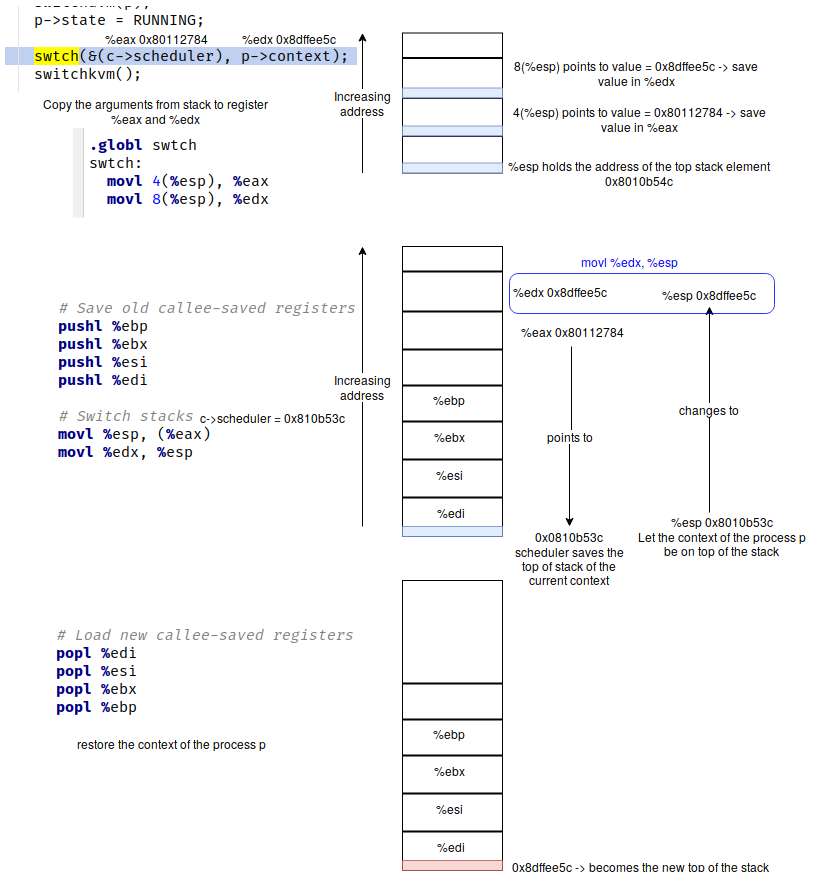
\includegraphics[width=\textwidth]{context_switch.png}
    \end{minipage}%
    \begin{minipage}[t]{0.5\textwidth}
        \vspace{-8cm} 
        \begin{itemize}[topsep=0pt, partopsep=0pt, itemsep=0pt, parsep=0pt]
            \item  When swtch function call is made, old kernel stack has return address (eip)
        and arguments to swtch (address of old context pointer, new context pointer)
        \item  Store address of old context pointer into eax
        \item  Store value of new context pointer into edx
        \item  Push callee save registers on kernel stack of old process
        \item Top of stack esp now points to complete context structure of old process
        \item  Update old context pointer (eax) to point to updated context
        \item  Switch stacks: Copy new context pointer from edx to esp
        \item  Pop registers from new context structure
        \item  Return from swtch in new process
        
        \end{itemize}
     
    \end{minipage}
    \caption{Assembly code in xv6 for \texttt{swtch()}}
    \label{fig:parallel}
\end{figure}

\subsubsection{\texttt{swtch()} for new processes}
Our way of working assumes the existence of a context structure of a process.
What if the process just started and has never run before (ie) a newly forked process?
The kernel stack of such new processes are setup\footnote{They are artificially setup with appropriate context sturcture and trap frame} in such a way that the EIP of function 
where the process starts from is saved in the context structure to mimic that the process
was switched out from where we want to resume in kernel mode(this location is just after the fork wherever our PC is pointing to). Apart from this the trap frame is copied
from the parent(\texttt{eax} or return value alone is changed for the \texttt{fork()}) so it has the proper \textit{register context} to resume in user mode just after wherever \texttt{fork()} call was made. Process resumes execution in kernel mode and it returns from trap to
user space(to the instruction right after the \texttt{fork()}).  


\textbf{allocproc:} This is the function that creates a new \textit{struct proc} for our newly forked process. It finds
an unused entry in the ptable and marks it as an embryo and changes it to runnable after the process completion is well "completed". It
also allocates a \textbf{PID} for this process along with new memory (ie) a kernel stack and also a stack pointer pointing to the bottom of this stack.
What else?
\begin{itemize}[topsep=0pt, partopsep=0pt, itemsep=0pt, parsep=0pt]
    \item Leave space for trapframe (copied from parent)
    \item after that pushes return address of “trapret”
    \item Push context structure, with \texttt{eip} pointing to
    function “forkret”. This is done since, when new process is scheduled, it begins
    execution at forkret, then returns to trapret, then returns from trap to userspace continuing to execute instructions after fork
    \item Thus we have hand-crafted kernel stack to make it look
    like process had a trap and context switch basically lying to the scheduler to make it like look like any process which was context switched in the past. So the OS scheduler can schedule it as it does
    any other process
\end{itemize}
\noindent\tbox{
    \begin{center}
    \textbf{\Huge Lecture 9}
    \end{center}
}

\subsection{OS Scheduling Policy}
Now that we have understood the mechanism of the OS scheduler let's see how the scheduler chooses which amongnst the 
ready processes it should run. An important point to note is that only when a process is in kernel mode for a trap a context switch happens. However not on every trap does the scheduler perform a context switch
The first classification among schedulers as we saw before are pre-emptive and non-premptive schedulers.
\begin{itemize}[topsep=0pt, partopsep=0pt, itemsep=0pt, parsep=0pt]
    \item \textbf{Pre-emptive:} Performs \textit{involuntary} context switches using timer interrupts\footnote{Refer \ref{section:Timer}}
    even if the process is in ready/runnable mode.
    \item \textbf{Non-preemptive:} Performs only voluntary context switches when a process gives up the control via a trap.
\end{itemize}

What are the goals of a scheduling policy?
\begin{itemize}[topsep=0pt, partopsep=0pt, itemsep=0pt, parsep=0pt]
    \item Maximise utilization: Efficient use of CPU hardware so that the throughput of the CPU is maximised
    \item Minimize the time it takes for a CPU to complete a process. It is also called as turnaround or completion time
    \item Minimize time it takes for the process to start running after it is ready to run which is called response time\footnote{Very important for processes that are highly interactive and constantly take input from users}
    \item Fairness is to be maintained (ie) all processes get a fair share of CPU (account for priorities also)
    \item We also want to minimize overhead. That is we don't want the scheduling itself to take too much processing power/time.
    We can't have unnecessarily large number of context switches (since it takes \(\sim \)1 microsecond to switch) or have too much time needed to take a decision even with larger number of processes to be scheduled
\end{itemize}


\subsection{Different scheduling policies}
\begin{enumerate}
    

    \item \textbf{FIFO(First in first out):}\\
    We put all our processes in a queue and then we run them one after another.
    Note that FIFO is non-preemptive (ie) a processes runs to termination or till it is blocked. In case of a blocked syscall, after it is done with handling
    a blocking syscall we add it to the end of the process as a new process with a new context. When it is added back it counts as a fresh CPU burst
    \footnote{A CPU burst is the time for which a process runs in a continuous stretch}

    \begin{table}[h]
        \centering
        \begin{tabular}{|c|c|c|c|}
        \hline
        \textbf{Process} & \textbf{CPU time needed} & \textbf{Arrives at end of} & \textbf{Execution time} \\
        \hline
        P1 & 5 & 0 & 1-5 \\
        \hline
        P2 & 3 & 1 & 6-8 \\
        \hline
        P3 & 2 & 3 & 9-10 \\
        \hline
        \end{tabular}
        \caption{FIFO}
        \label{tab:FIFO}
    \end{table}
    The disadvantages with FIFO is the convey effect (ie) processes which are shorter tend to get stuck behind much longer ones resulting in unnecessary increase in the turnaround time due to longer waiting time
   \item \textbf{Shortest Job First(SJF):} \\Asssuming that the scheduler has the knowledge on the CPU burst of all processes (time it runs for one continuous stretch). 
    Now we can pick the process with the shortest burst time first and run it and continue doing so. This can be done by maintaining all the processes
    in a heap ordered by burst time needed.
    \begin{table}[h]
        \centering
        \begin{tabular}{|c|c|c|c|}
        \hline
        \textbf{Process} & \textbf{CPU time needed} & \textbf{Arrives at end of} & \textbf{Execution time} \\
        \hline
        P1 & 5 & 0 & 1-5 \\
        \hline
        P2 & 3 & 1 & 8-10 \\
        \hline
        P3 & 2 & 3 & 6-7 \\
        \hline
        \end{tabular}
        \caption{Shortest Job First}
        \label{tab:SJF}
    \end{table}
    This can be proved to be the optimal solution when we assume all the processes arrive at the same time. However this is an unrealistic assumption.
    Also due to its non-preemptive nature short jobs can still get stuck behind longer ones (different arrival times). 

    \item \textbf{Shortest remaining time First(SRTF):} This is a preemptive version of \textbf{SJF}. A newly arrived process can preempt\footnote{terminate this process and make CPU context switch to itself} a running process, if 
    CPU burst of new process is shorter than remaining time of the running process. This avoids the problem of shorter process getting stuck behind longer ones if they don't arrive at the same time.
    
    \begin{table}[h]
        \centering
        \begin{tabular}{|c|c|c|c|}
        \hline
        \textbf{Process} & \textbf{CPU time needed} & \textbf{Arrives at end of} & \textbf{Execution time} \\
        \hline
        P1 & 5 & 0 & 1,\textit{preempted} then 7-10 \\
        \hline
        P2 & 3 & 1 & 2-4 \\
        \hline
        P3 & 2 & 3 & 5-6 \\
        \hline
        \end{tabular}
        \caption{Shortest Remaining Time First}
        \label{tab:SRTF}
    \end{table}
    However we are still assuming knowledge on the run times of processes before they arrive (unrealistic assumption).
\item \textbf{Round Robin(RR):}\\ This is the first practical policy we are seeing. We fix a time slice (called a quantum). The quantum is a multiple of the length of the timer interrupt.
So when the time interrupt happens the scheduler checks if the process has already run for the allocated time slice. If that is not the case, control is simply handed over back to the process. If not so, control is handed to another
runnable process by context switching into it. Thus the timer interrupt is used to enforce periodic scheduling. 
This policy is good for maintaining both response time and fairness, however it is not the most efficient for turnaround time. \texttt{xv6} uses this policy

What effect does time slice's length have?
\begin{itemize}[topsep=0pt, partopsep=0pt, itemsep=0pt, parsep=0pt]
    \item A small time slice makes it inefficient since too many context switch happen and the time spent to context switch isn't \href{https://english.stackexchange.com/a/138566}{amortized} properly
    \item If the time slice is too big there is no responsiveness as one process hoards the cpu for a longer time
\end{itemize}

\item \textbf{Weighted Fair Queueing(WFQ):} \\This is a modified version of Round Robin policy. We set weights to every process and give preferences according to it.
The weight setting is done by both user and the OS itself to different extents. The time slice is for a given a process is proportional to this weight. Real life schedulers may not be able to maintian the time slice enforcement accurately. Think about cases where the time interrupt
doesn't align with time share or a process is blocked before its slice. A practical modification to accomodate such things is to keep track of the run time of a process and switch in the process which has used the least fraction of its fair share. This compensates for deficiences/excess in the running time.
 
\item 
\textbf{CFS scheduler}:\\The Completely Fair Scheduler used in linux is a variant of WFQ. It uses red-black to keep track of who all runs and keeps track of who all have used up least amount of their fair share.
However it is impossible to be fully fair whilst being reasonable but this policy is close to optimal fairness.


\item \textbf{Multi-level feedback queue (MLFQ):} \\
This is another practical algorithm with realistic assumptions. We would prefer the property of the SJF which gives priority to smaller jobs. However we can't assume we know the running time before.
We also want to ensure that the response time is lesser as we see in Round robin. 

We have multiple queues corresponding to multiple priorities. Scheduling of processes happen first for higher priority queues and within a queue Round Robin is used for scheduling. If a process has used up more of its fair share of CPU we decay it's priority and push it down. When we 
add a process we add it to the high priority queue. This helps us have an idea on which process is running for a longer time and which ones haven't. We run and finish up shorter processes quickly (Like I/O) even without prior knowledge of CPU bursts. Periodically reset the priority level to make sure even longer
process gets some chance to run.

Note that processes in lower priority queues are never done unless higher priority queues are empty. What to do if a process yields CPU just before its fair time is over?? Do you
reset the time? Doing this would create a possible attack on the CPU resources wherea processes calls an empty IO just before its time slice is over thus remaining in the highest priority queue. We must
account for the total time a process ran for to avoid this. 
\end{enumerate}

\newpage
\noindent\tbox{
    \begin{center}
    \textbf{\Huge Lecture 10}
    \end{center}
}

\subsection{Multicore Scheduling}
Scheduling decision is supposed to be made seperately for each core. Do we bind a process to a particular CPU core always or do we let a process,
run on any CPU core that is free? Making sure that the process runs on the same core as much as possible is better due to improved CPU cache performance.
However balancing is important, if the core is highly overloaded then we ensure a process runs on a different free core to not waste time. 

Overall however having
a single queue which assigns the ready process to the first free CPU out of all of the multiple CPU's present is more efficient than having
multiple queues for each CPU and choosing to put a process in one of these queues. This is due to the high cost and thus inability to switch queues once a process
is assigned a queue in the multiqueue case.

x
\section{Inter Process Communication}
Why do we need IPC\footnote{Interprocess Communication}? In real life systems it is not ideal or feasible to maintain all of the functionality in just a single
process. Rather we 
modularise code (which can be in different languages, frameworks and written by different teams of people) and need some method for them to work along with each other.

Processes in a system needn't share memory with each other by default. However they still need the ability to communicate. This is done via
IPC mechanisms, which are available via the OS whcih provides several syscalls enabling the exchange of information between processes. The communication can also
be done by two processes agreeing to share a particular portion of the memory image to enable communication. Communication can also be done by having a particular
memory area (buffer) specifically meant for communication. It is important to note that it is an extremely dumb idea to just let two processes have access to the entire 
memory images of each other since this destroys the ability to maintain isolation of processes.   


\subsection{Sockets:}
Sockets are an abstraction to enable communication between processes. Each process opens its own socket and two sockets of two processes can be connected.
The process to open the socket first is the \textit{server} and the process which connects its socket to the server is the \textit{client}. A socket is a way of 
bidirectional communication, thus a process can write into its socket which can be read by other processes and vice versa. Processes communicating using socktes can be 
in the same machine or on different machines. While communicating on the same machine the buffer\footnote{intermediate storage which stores message to be sent} is present in OS memory. For communicating across machines messages are sent on the network.
\textit{Unix Domain sockets} are used to communicate between processes on the same machine. \textit{Internet sockets} are used to communicate between
processes on different machines. 


The client needs some information about the process whose socket it wants to connect to (server). Thus every socket needs a unique number
to identify itself. This \texttt{ID} for a Internet socket is the IP address and port number. Local sockets are identified a unique \textit{pathname} identifying it in the local machine. Note that the local
socket isn't exactly a file but it has a pathname that only serves the purpose of identying it uniquely.
The server needs to publicise its identifier (IP or pathname) for the client process to know where to connect to.


\textit{Connection-based sockets} are those when a client and server are explicitly connected to each other. After this connection they can only talk to each other. So there is no need to explicitly mention which socket we want to communicate to.
\textit{Connection-less sockets} are those who can communicate with multiple processes at the same time. Thus we need to mention the address of the socket we want to communicate with. 


\subsubsection{\texttt{socket()} syscall}
The \texttt{socket()} syscall is used to create a socket. It takes the type of socket as an argument and returns the file descriptor of the socket to the process. This file descriptor 
is used for all operations on the socket by this process. A socket can optionally bind to the address (pathname or IP address/port number) using \texttt{bind()} system call. 
Server socket binding means that the socket is given a global address which can be used by other processes to communicate to this socket. Note that binding is compulsory for server sockets who need to 
publicise this binding address to enable clients to talk to them. The \texttt{close()} system call closes a socket.


How do processes use \textbf{sockets} to communicate?
\begin{itemize}[topsep=0pt, partopsep=0pt, itemsep=0pt, parsep=0pt]
    \item \textbf{sendto():} is used to send a message from one socket to another connection-less socket. It takes its own socket's file descriptor, the message to be sent, the other socket's address as arguments
    \item \textbf{recvfrom():} is used to recieve a message from a socket. It takes the its socket's file descriptor, a message buffer to copy the message into and a sockets address structure into which the sending socket's
    global address is filled. Now this process can use the address it just obtained to communicate back to the process which sent it a message. 
\end{itemize}

\noindent\tbox{
    \begin{center}
    \textbf{\Huge Lecture 11}
    \end{center}
}
\subsubsection*{Connecting sockets}
Connection-oriented sockets need to be explicitly connected for transfer of messages.
After a server binds to a well-known address\footnote{gets assigned a proper global address}, it uses the \texttt{listen()} syscall to listen
for "requests to connect" from clients who want to connect to server. Clients use the \texttt{connect()} to send a request to connect to the server. The server
uses \texttt{accept()} syscall to accept a request from the client to establish a connection. Once an \texttt{accept()} syscall is sucessfull then a connection
is established between the client and server. 


The \texttt{accept()} syscall takes the file descriptor of a socket as an argument. This socket's address is what clients use to send a "request to connect".
Once the \texttt{accept()} syscall is succesful it returns a \textbf{new file descriptor} to a socket which is connected to the client. This new socket is different from the \textit{listening socket}

Hence it is important to note that there is a \textit{listening socket} corresponding to whose address requests are send to connect and there are (possibly multiple)
\textit{connected sockets} explicitly connected to a client socket to enable communication between two unique processes. 
The \texttt{accept()} syscall will block the server till is recieves a request to connect from a client. Similarly, the \texttt{connect()} syscall blocks the client till the server accepts the requests.

After a client connects to a server, the \textit{pair of sockets} are used to exchange data. Again let's reassert that the \textit{connected socket} is the one which is used to transfer messages not the \textit{listen socket}.
Syscall \texttt{send/write} to send a message which only goes to the connected socket.
Similarly syscall \texttt{recv()/read()} is used to recieve a message on connected socket. 
The arguments given to send/recv are the socket fd, message buffer, buffer length and (optional) flags.
The return value is number of bytes read/written or error number.
We need not specify socket address on every message, as they connected already and only communicate with each other using that particular socket.

In any kind of real system multiple connected and connection-less sockets connect multiple processes in several ways forming a complex network of processes all working with one another to achieve some task. 

\subsection{Message queues}
Message queues are another method used for exchanging messages between processes. We open a connection to a message queue identified by a "key", and get a file descriptor to it. The sender can open a connection to
the message queue and send a message. The reciever opens a connection to the message queue and recieves the message later on. The message queue acts as a buffer till the message is retrieved by a reciever.


There are three main syscalls associated with a message queue:
\begin{itemize}[topsep=0pt, partopsep=0pt, itemsep=0pt, parsep=0pt]
    \item \texttt{msgget()}: syscall to get the id of a message queue. The parameters it takes are the key of the message queue . It returns the msg\_queue identifier (a file descriptor) on success and -1 on failure.
    \item \texttt{msgsnd()}: The parameters it takes are the msg\_queue identifier and the message to be sent and its size. It returns 0 on success and -1 on failure. 
    \item \texttt{msgrcv()}: The parameters it takes are the msg\_queue identifier, size of the message and the buffer to write the message into. It returns the number of bytes recieved on success and -1 on failure.
\end{itemize}
There can be several different message queues all with their own unique "keys". Also note that multiple processes can use the same message queue if they all have access to its key. Thus we need to be careful about which process's message is being recieved when \texttt{msgrcv()} is used.

\subsection{Pipes}
A pipe is a unidirectional FIFO channel into which writing is done on one end and reading from another end. The syscall \texttt{pipe()} is used to create au unnamed unidirectional pipe. Named pipes are made using \texttt{mkfifo()}. It returns two file descriptors for 
the end points (one for write, other for read). A pointer to a \texttt{struct} of a pair of numbers are passed as a parameters of the pipe. Once a pipe is succesful this \texttt{struct} has both file descriptors. Why do we have access to both descriptors? This is because Pipes
are frequently used for communication between a parent and a child. The data written into a pipe is stored in the buffer of the pipe channel until they are read. Obviously, bi-directional communication between two processes needs two pipes. 


\textbf{Anonymous pipes} are only available to communicate between process and its children. The pipe file descriptor is available to both the parent and the child.

\textbf{Named pipes} are used by two unrelated processes to talk to each other. The pipe is opened with a pathname which is accessible across processes. One of the processes
has access to the read end of a pipe, while the other other process opens the write end. 


\textbf{Buffer Mechanism:}  
When we want to send a message the general mechanism stays the same across all these sycalls. We write the message into a temporary space called the buffer. This buffer is usually some memory location
inside OS not directly accessible by the user.
In all of these system calls the buffer maintains the messages in a FIFO order. When the buffer is read the message which was in it and was read is cleared. Sender 
usually can't be blocked by \texttt{send()} syscall unless the temporary buffer is full. Similarly reciever can be blocked if temporary buffer is empty. We can also customize the sycalls to not block the process
but return some error code for us to handle to error manually.

\subsection{Shared memory}
Processes in a system do not share any memory unless mentioned otherwise. Child process \textit{copies} the memory of the parent but doesn't share the memory image.
Shared memory means that the same memory image appears in multiple processes. Each memory \textit{segment} shared is identified by a unique key. A process can request to map/attach this shared 
memory segment into its own memory image using this identifier key. 

Sharing of memory is a risky and volatile task. The processes thus need extra mechanisms to know for example, if the memory has been modified. This enables them to coordinate with one another

\newpage
\noindent\tbox{
    \begin{center}
    \textbf{\Huge Lecture 12}
    \end{center}
}
\part{Memory Management}
\section*{Abstraction of Address space}
Every process assumes it has access to a large space of memory from address 0 to a max value. The maximum value depends on the available number of bits for the memory space.
The virtual address sapce contains all the code/data that a process can access. Addresses in CPU registers point to these virtual addresses.




However this is not how memory is actually stored. The OS maintains this illusion of virtualized address spaces by having a map from every virtual address to a physical address. When the CPU accesses memory 
using an address (virtual address) the Memory Management Unit (MMU) converts it to a real address and gives back the data at the physical memory corresponding to the virtual address. OS allocates physical memory to a process, it has the translation information
provides it to MMU.

Why do we need the MMU? Why not the OS? This is primarily since we don't want to trap into the kernel for every memory access. The OS does the background work
of allocating memory for processes and maintaing the virtual address $\rightarrow$ physical address mapping and simply passes on the information to the MMU.
The MMU deals with translation of virtual memory to real memory. During Bootup the OS starts on the MMU and starts giving it translation information.
\begin{figure}
    \begin{center}
        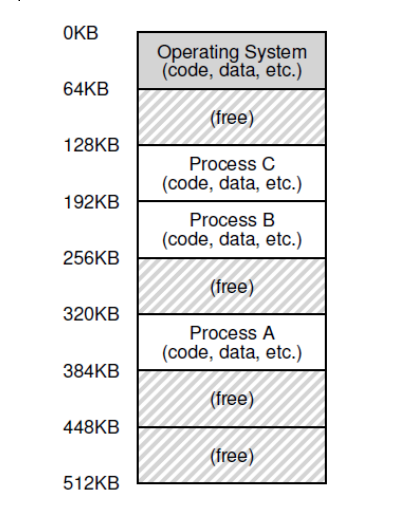
\includegraphics[width = 6cm]{memory_allocation.png}
        \label{figure:memory_alloc}
        \caption{Memory allocation for three processes}
    \end{center}
\end{figure}


\subsection*{Why virtual address?}
The real view of memory is messy and it is not easy to manage manually. In earlier systems there was only one process and its own code. Nowadays we have multiple
parallely running processes which all do time\-sharing on the same CPU. Memory is also allocated in a non-contiguos manner, but we still want to maintain the illusion of memory being continuosly allocated. 
Thus virtualization has become a neccesity in modern systems. The CPU \textbf{only} uses the virtual addresses to perform any action.\footnote{For example addresses of a pointer obtained from \texttt{malloc()} is the virtual address}

\section{Base and bound}
This is the simplest form of memory management. It is not used in modern systems but we will understand it to get some insights. The memory image
from [0,N] is placed at memory address base B. That is every virtual address X is stored at physical address B + X. There is also a bound associated with this base which tells us 
the maximal address for the memory allocated in this memory image.



Simple example: Let's take a small program as given hello

\begin{lstlisting}
    void func(){
        int x = 300;
        x = x + 3;
    }
\end{lstlisting}
This code compiles to give instructions. 

Suppose the OS places the entire memory image in one chunk starting at physical address 32kb, then the OS indicates base and bound to MMU. 
MMU performs this translation from Virtual adress to physical address. But what if some garbage address/ out of bound address is given? Then the
MMU raises a trap to call the OS to handle this situation. This is another type of hardware level trap (program fault). In this case int n is inserted into the 
stream of instructions run by the CPU. 

\section{OS vs MMU}
The OS is the one who allocates the memory and builds the translation information of a process. However the MMU
is the one who translates virtual address to a physical address. Note that once the user starts running the OS is out of the picture unless there is a trap.

When a context switch happens the OS changes the translation information in the MMU to enable it to perform translating addresses corresponding to this new process \footnote{same virtual address means different physical address in different processes}. 
As told before when the CPU has an instruction which wants to access memory the MMU translates it to a physical address which can be used to access the data.

\section{Segmenation}
It is an upgradation of base and bound. The program is split into several segments (Code, data, stack) and each of them is placed at a different memory location (base).
Each of these bases also have a bound associated with them. When the address exceeds the bound of a segment we obtain a \textit{segmenation fault}\footnote{\href{https://www.youtube.com/watch?v=NAEppFUWLfc}{\textit{sigh}}}
. Thus when we context switch into a process the OS updates the MMU with all the necessary bases and bounds.
Each virtual address is hence a segment identifier bit sequence concatenated with an offset for that particular byte.

But this is still inefficient due to the variable sizes of these segments. This also results in \textit{fragmentation} where there is some unusable space between two segments. 

\section{Paging}
Paging is the mostly widely used system of memory Management today. We divide our virtual address space into fixed size pages. Each one of these pages is assigned a free \textbf{physical frame}\footnote{Just the physical memory associated with a single page}.
The memory allocation for each page is done at a fixed size (eg. 4kb). Since the pages are tightly packed we have no wasteage of size between pages (ie) no \textit{external fragmentation}. However inside the pages we could have some wasteage of space (ie) \textit{internal fragmentation}.

What is the optimal page size? Why 4kb?
\begin{itemize}[topsep=-5mm, partopsep=0pt, itemsep=0pt, parsep=0pt]
    \item \textit{Large page size} \(\rightarrow\) larger amount of wastage inside individual pages.
    \item \textit{Small page size} \(\rightarrow\) OS has to keep track of huge number of pages which creates a large overhead.\footnote{Large processing power is needed to maintain page table}
\end{itemize}
\newpage

\noindent\tbox{
    \begin{center}
    \textbf{\Huge Lecture 13}
    \end{center}
}
\section{Page table}
\subsection*{What is a page table?}
The page table is a per process structure (ie) each process has its own page table. This table helps to translate
virtual addresses to real ones. It stores frame numbers for all the pages used by the process in an array format. 
Table[i] gives the physical frame number of the ith virtual page of the process. Thus the ith entry of the page table corresponds to the physical address of the starting byte of the ith page. The page table is stored in a part of a OS memory (stored in PCB). The MMU has 
access to the page tables of current processes and it uses it for translation. 


Given page table of a process, how is physical address obtained from virtual address?

When you have the virtual address you can find which page your data is in. This can be done by (Virtual Address / Page size) and the offset is (Virtual Address \% Page size).
That is the most significant digits give the page number and the least significant ones give the offset. 

\begin{figure}
    \begin{center}
        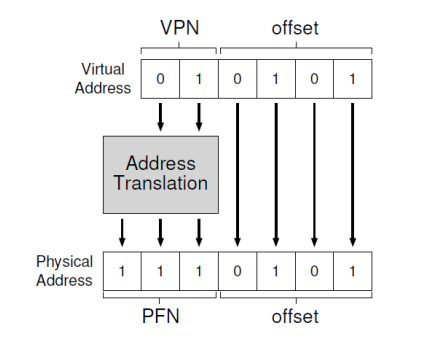
\includegraphics[width = 6cm]{address_translation.png}
        \label{figure:address_translation}
        \caption{Visual representation of address translation}
    \end{center}
\end{figure}


Hence the most significant digits give the Virtual Page Number (VPN) and least significant bytes give the offset. The VPN and the page
table can be used to get the Physical Frame Number. Note that Page\_Table\_array[VPN] = PFN\footnote{Physical Frame Number}. Obviously the offset to get the byte
we want is same in both the Physical frame and the virtual page.

\subsection*{Translation Lookaside Buffer(TLB)}
An important point to note with paging is that one memory access has become two accesses now. One access to the page table and the one to the actual byte we want. This results in a significant
slow down since memory accesses are very slow. This is the overhead associated with paging.

To reduce this overhead the MMU caches the most recent translations in translation lookaside buffer(TLB)\footnote{It is a fully associated cache}.
TLB caches only the \textbf{page table entries} \footnote{the physical data in 32/64 bit addresses are cached by the actual cpu cache}. If we have
a hit, we fetch the memory contents of the given address in one access since we already have the page table entry in the cache. If there is a miss we get the memory from RAM and place it in TLB for future accesses after 
which we use the translated address and then again use this page table entry to translate the virtual address and get the memory we wanted.

Interestingly, during a context switch the TLB is flushed. This is due to the fact that the MMU needs to translate the Page table for every processes in a different
way (different page table entries).


Thus the TLB is very important and \textit{needs} to have a high hit rate. It works 
parallely with the CPU cache to further optimize memory accesses.  
\\

\newpage
\noindent\tbox{
    \begin{center}
    \textbf{\Huge Lecture 14}\\
    \end{center}
}

\section*{Page table entries}
As we saw before the page table is an array of page table entries. 
There are a large number of virutal pages available but each process only uses a few. Thus to indicate that
a virtual page is not used each page table entry of a page table has a \texttt{valid} bit. If this bit is 0 that entry is invalid and if it is 1 then it is used. 
The invalid page table entries in a process can be used by some other process at the same time. So not being able to access these entries is extremely important for isolation purposes.

We also have other similar \textbf{permission bits} which we will look at later.

The number of bits in the virtual address corresponding to the offset of a particular page is dependent on the size of the page. 
If the size of the page is say x bytes then the number of bits required for offset is \(\log_{2} x\)\footnote{12 bits in 4kb case}. The remaining bits of the address are used to indicate the 
Virtual Page Number. If the Virtual Page number does not correspond to a valid entry of the page table then the MMU raises a trap (it is an out of bounds access). Thus the most significant bits are used as an index to get the Physical frame address from the 
page table and the remaining bits are the offset to get the actual memory byte we want to access. 

In a 32 bit (4GB) system usually, a page is 4kb large. There are (1024 * 1024 pages (ie) around a million pages) in a page table.
\section*{Inner and outer page table}
The page table is of size 1MB (All 32-bit addresses are stored). But we know that the size of the physical frame which is the size of an available contiguos memory chunk is 4kb. 
So how is the page table stored?. Interestingly the page table is divided into 1024 inner page tables which have their start addresses in another "outer" page table corresponding to each inner page table. To reiterate, each of those 1024 byte sized chunks of the page table is an inner page table.
This outer page table has a size of 1kb (Since each page table entry covers 1024 bytes corresponding to one inner page table). 
This solves our limitation in the size of our physical frame. The outer page table is as powerful as the normal page table which comes into use.


\begin{figure}[h]
    \begin{center}
        \hspace{2cm}
        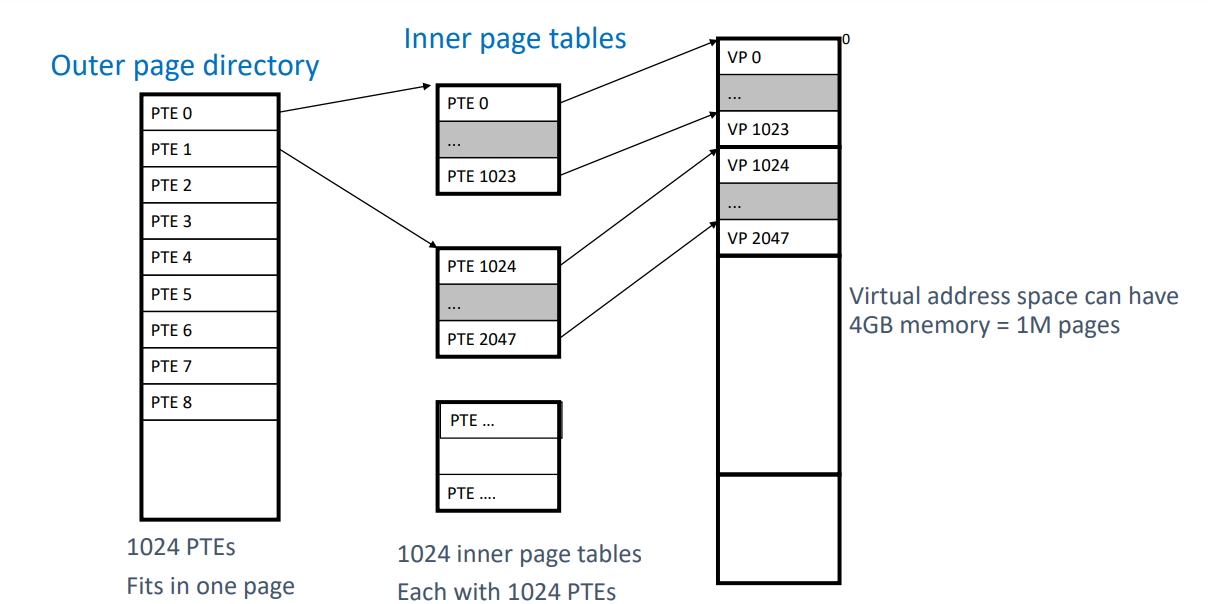
\includegraphics[width = 12cm]{inner_page_table.png}
        \label{figure:inner_page_table}
        \caption{Mapping from outer page table to inner page table }
    \end{center}
\end{figure}

Say we have a process which has 2k pages needed for code and data and after that it has 6k unallocated pages and then 1k unallocated pages (for the stack) followed by the stack itself\footnote{Note that }.
Here if we had entries for all pages in their corresponding inner page table with valid/invalid bits it is easy to see that it is a lot of work since we need to bother about 1024 * 1024 entries. A smart solution is, rather
than worrying about the inner pages tables at all just set an entry of the outer page table to be invalid iff all the entries in the inner page table corresponding to it are not used. Thus instead of setting 1024 entries of the inner page 
table to invalid we directly make the outer page table entry corresponding to all of them invalid. Hence we need not even bother creating/maintaing inner page tables with no valid entries.



As a conclusion, in our paging system there are 4GB bytes which are split into 1M pages of size 4kb each. There are 1M entries in the page table corresponding to each virtual page. The 1M entires of the page table are divided into 1024 inner page tables.
The inner page table has the physical frame address corresponding to a virtual page. Each of these inner page tables is mapped to an entry in the outer page table thus the outer page table has 1024 entries.



\subsection{Multi-level Page Tables}
How are addresses translated in a two level Page table? As we saw before the most significant bits denote the page number. Now we can even split these most
significant bits into two parts where the more significant bits represent the index of the outer page table whereas the one less significant represent the offset within the inner page table to get the appropriate page table entry. Thus to get the actual 
physical address the MMU walks along the page table arrays. This is why the MMU accessing the page table is called walking the table. 


MMU stores starting, physical address\footnote{Since we need the actual access to the page table} of the page table in a single level page table or specifically the outer page table incase of multi-level paging. 
This is stored in the page table base register of the MMU.

What if splitting into two levels isn't enough? This process of making page tables for page tables can be continued up until the final/outermost page table can fit within a single page. 
However this comes with the obvious overhead of making each page table walk longer and thus more time consuming. 

\newpage
\noindent\tbox{
    \begin{center}
    \textbf{\Huge Lecture 15}\\
    \end{center}
}
\vspace*{0.1cm}


As an example consider a 48-bit cpu architecture with pages of 4KB size. Thus the number of pages will be \(\frac{\text{Total number of bits}}{\text{Size of a page in bits}}\) (ie) \(\frac{2^{48}}{2^{12}}\) so \(2^{36}\) pages. So we need an array to store the corresponding 
physical frame address for each virtual page that is \(2^{36}\) entries. Now obviously this innermost page table isn't less than the size of one page which is \(2^{12}\). Hence it can't be stored continuosly in a single page and we need to find futher divide the table into page table sized chunks and map each of them to a physical frame address.
So lets do make a page table for the inner most page table. From similar caluculations the size of this new table will be \(\frac{2^{36}}{2^{12}}\) which is \(2^{24}\). This again isn't small enough to fit in one page. Let's divide again. Now we have \(\frac{2^{24}}{2^{12}}\) which is \(2^{12}\). Finally this is exactly one page long.
Thus we stop.

We ended up having 4 levels of page tables here. The size of the innermost page table entry is \(2^{36}\), so 4-byte (32 bit) addresses are not enough to identify each entry uniquely thus we have 8-byte addresss.  The most significant 36 bits help us get the physical frame address of each page and the remaining 9 bits give the offset.
Now among these 36 bits the first 24 tell us the physical frame address of the beginning of a chunk into which the inner most page table is divided and the 9 bits give us the offset among one such chunk. Reiterating that the innermost page table is divided into \(2^{24}\) chunks and each of this is mapped to a page. We can continue in this way to 
index each element of the tables at every level when given a 48-bit address.
 
\begin{figure}[h]
    \begin{center}
        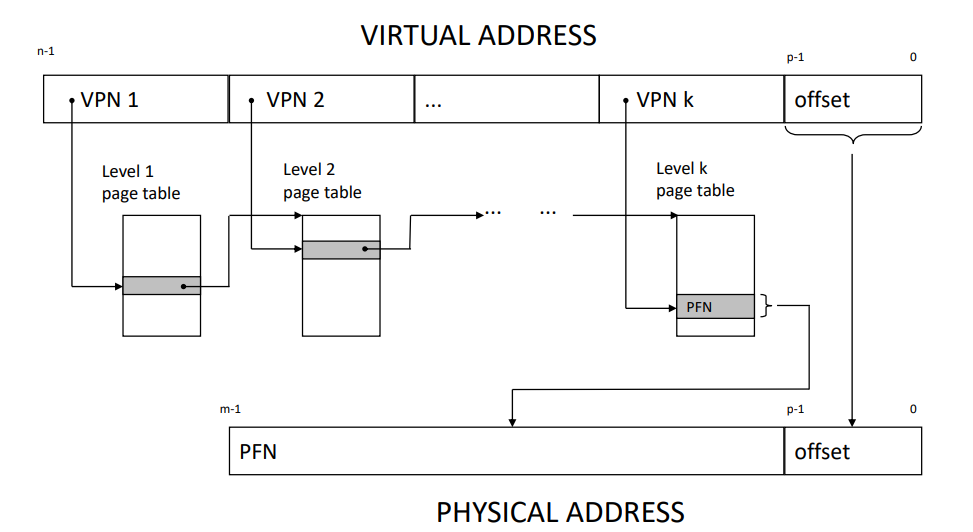
\includegraphics[width = 12cm]{mulit_level_page.png}
        \label{figure:multi_level_page_table}
        \caption{Translation from multi level page table to physical address }
    \end{center}
\end{figure}

\section{Virtual Addresses}
It is important to note that every element of memory needed by a process has a virtual address associated with it. This is due to the fact that MMU can access elements only via
virtual addresses. So every element like the code, data has a virtual page and a mapping to its physical address. Even libraries that we import or the OS is mapped to a virtual
page by \textbf{each} process.

What virtual addresses are given to the OS,libraries which are not technically part of the code? We give such elements \textit{high virtual address}. This is done to prevent accidental
collisons in the virtual addresses assigned to these elements and other things like stack, code, data. Note that this does not mean each process has a copy of the OS, libraries. Rather each process
has an entry in its page table and thus allocates virtual pages to these elements, however the physical addresses these virtual pages point to \textit{remain the same.}

Also thinking the other way around anything inaccessible by a process is not part of the virtual address space. 

\section{OS is not a process}
From the discussion above one important point to notice is that the OS isn't a seperate process with its own address space. The OS is mapped for each process to be a part of its virtual memory.
This denotes a very important point established in the beginning of the course. \textbf{Each process thinks it owns the system.} Each process thinks it is the only one existing and that
it has a monopoly over the system and that the OS code is a part of it.

When the Bootloader runs, it places the OS memory in the very beginning addreses of the ram. Thus the OS has high virtual address and low physical addresses.'

\subsection{Permission bits}
\label{section:Permission bits}
How is illegal OS access prevented? As we saw before we have permission \texttt{bits} which can make a page table entry invalid, make a page read( or write ) only, make it accessible only during user mode etc. 
Thus the OS page table mappings have permission bits to allow access only in kernel mode. Similarly our code's pages are assigned read only privileges since we do not have to change instructions after compilation. 

\subsection{Memory management in xv6}
xv6 has a two level page table system. It has 1024 inner page tables with 1024 entries corresponding to each of them in the 
outer page table. The physical address of the base of the outer page table is put in the CPU's cr3 register, which is used by the MMU
during address translation.

The size of the virtual address space in xv6 is 4GB. The physical address space ranges from [0,PHYSTOP]. \texttt{PHYSTOP} is a macro to denote
the maximum size of the usable physical address in xv6.



























\noindent\tbox{
    \begin{center}
    \textbf{\Huge Lecture 16}\\
    \end{center}
}
\section{Demand Paging}
Now, think about if it is necessary to have all the pages in the main memory? This is not necessary as a process can't use them at once. This is
also not possible with larger address spaces. Modern operating systems provide only virtual memory. That is not all logical pages are assigned physical frames.
Even those that are, are not permanently kept in main memory. Some pages are stored in disk and brought to main memory \textit{on demand}. This is called 
\textbf{Demand paging}. \footnote{Demand Paging is not present in xv6}

\subsection*{Swap space}
This is the special area in the disk to hold pages that do not fit in DRAM. Pages are pushed
to the swap space when the main memory (DRAM) is full. This is brought into memory when a page is accessed.

Recall valid bits. If a page is invalid we don't store any frame number for them. However for valid pages we either store the physical frame number or 
a disk address space. Now we also need to denote if an entry contains a disk addreses or a physical frame address. For this purpose we have a permission\footnote{Refer \ref{section:Permission bits}} bit called
the present bit. If the present bit is 1 then the memory is in DRAM else it is in disk space.  

\begin{table}[h]
    \centering
    \begin{tabular}{|c|c|c|}
        \hline
        Valid & Present & What it represents\\
        \hline
        1 & 1 & The page is valid and in DRAM\\
        \hline
        1 & 0 & The page is valid and is in disk\\
        \hline
        0 & 1 & Stupid, doesn't happen\\
        \hline
        0 & 0 & Invalid page\\
        \hline
    \end{tabular}
    \caption{Table to show valid, present bit configurations}
    \label{tab:present_valid}
\end{table}

Note that in mulitlevel paging we can still have some of the pages in DRAM and some of them in disk.
From the above discussion we can see that the OS \textit{overcommits} pages (ie) tells the process it has access 
to a lot more pages than it actually does and it takes care of giving these pages by getting them from disk \textbf{on demand}



\subsection{Page faults}
When the MMU walks the page table to translate an address to a physical address, the various permission bits of the page table are also examined. 
If the MMU notices some unexpected behaviour it raises a trap and gives control to the OS.

Possible errors raised by MMU:
\begin{enumerate}[topsep=0pt, partopsep=0pt, itemsep=0pt, parsep=0pt]
    \item \textbf{Segmenation fault:} Trying to dereference some address of an unallocated virtual address. That is accessing memory which doesn't belong to the program. The OS kills the process in this case.
    \item \textbf{Illegal action:} The code performs some illegal action like attempt to access a page table that is not valid, or an attempt to modify a read-only page which obviously terminates the process.
    \item \textbf{Page allocation in DRAM:} When a valid bit is set but present bit is not set (page in disk), then OS allocates a page in the DRAM, updates the page table and then gives control back to the process.
    The process won't terminate in this case since the error was on the OS's side. Rather after handling the allocation process continues to run.
\end{enumerate}

\subsection{Reclaiming Pages}
The OS keeps track of all the free pages that are not being used so that they can be used during a page fault \footnote{The third type of fault}. If there is no free page available for the OS,
then it evicts a \texttt{vicitm page} and then pushes it from memory to the swap space (page table is updated). After this the page just freed up in the DRAM is allocated
for the page which raised the fault. 

We need to have a policy to determine how to choose a victim page. Note that the victim page can be in the same process or a different process.  

\subsection*{File backed, anonymous, dirty pages}
Pages in the memory image of a process are of two types.
\begin{itemize}[topsep=0pt, partopsep=0pt, itemsep=0pt, parsep=0pt]        
    \item \textbf{File-backed pages:} This contains data that comes from a file on the disk. (e.g Page with the executable code). So even if the memory in the DRAM is lost we have the file saved in the disk
    \item \textbf{Anonymous Pages:} These are pages containing data which are not stored anywhere. Some examples are the stack, heap. So if these are removed from DRAM they are gone forever.
\end{itemize}

File backed pages are further classified as:
\begin{itemize}[topsep=0pt, partopsep=0pt, itemsep=0pt, parsep=0pt]
    \item \textbf{Dirty Pages:} These are file backed pages whose contents is different from their copy on the disk.
    \item \textbf{Non-Dirty Page:} Pages which are identical to their copy on the disk.
\end{itemize}

This classification is kept track by the page table, again using permission bits \footnote{eg. the dirty bit}.
Why do we need this classification? We need to deal with page faults differently depending on which type of page it is.
When we reclaim memory from a victim page, we need to copy its content since it has changed compared to the file from which it came iff it is a dirty page. Else we can simply delete the page.

When we allocate memory during a page fault, the free memory frame must be intitialized with the content from the disk for 
a file backed and non-empty anonymous pages. For empty anonymous pages we just give an empty page for it. 

Note that a process maybe blocked quite a few times for disk I/O during a page fault. The average memory access time shoots up greatly if we have too many page faults. 

\subsection*{TLB and address translation}
Just a recap of how addresses are dealt with. The CPU only had virtual addresses which it deals with. The processor
requests the corresponding physical address from the MMU which looks in the TLB for an entry. If we have a hit/match for that address, the 
physical address is directly returned. Else the page table is walked and the entry corresponding to this Virtual address. This entry is used to get the 
address from memory. This address is also populated into the TLB for future use.     
\newpage
\noindent\tbox{
    \begin{center}
    \textbf{\Huge Lecture 17}
    \end{center}
}

\section{Thrashing}
We have several causes for an application to slow down but a page fault is an important reason for a massive decrease in efficiency. 
So it is essential that we have a large enough working memory to avoid page faults. 

Every process has a working set which is the number of frequently used pages in the memory image. The actual set of pages can change from time to time
depending on what process is running. This is usually smaller than the total virtual memory of the process. If we allocate memory lesser than the
size of the working set, we have frequent page faults.

Thrashing is this scenario where the system spends too much time servicing page faults and swapping back and forth from disk, and too little time doing
application based work. A fun example to think of to understand this is to assume that you want to study but you keep switching subjects every minute. Most of your time
goes off in taking and putting back books. 

The way to deal with Thrashing is to create efficient processes that don't use that many pages at the same time and also for the OS to terminate some processes.




\section{Page replacement policies}
We need to decide which page is our victim page we want to replace when the DRAM is full. Hence we need a replacement
poilicy

Some of them are
\begin{itemize}[topsep=0pt]        
    \item \textbf{Optimal policy:} We have 4 pages which the process needs but the process has space only for 3 pages in the DRAM. We assume that we can "look" into the future 
    and then evict the page which is not needed for the longest amount of time in the future. This ensures minimal number of misses. Obviously it is not implementable since we are not oracles
    who can look into the future.
    \item \textbf{FIFO:} We evict the page which was first put in the DRAM (ie) first page which was put in chronologically and then we evict that page. Bad idea since pages first put in are generally reused often
    
    \textbf{NOTE:} Beleady's anomalies are very weird examples of some policies doing worse on some inputs when they have more resources.
    
    \item \textbf{LRU:} The page which was accessed the farthest time in the past is evicted. That is if a page was accessed recently it is kept
    .The logic behind the policy is intuitive since a page accessed recently is much more likely to be accessed again.

    LRU \textit{seems} to be very easy to implement. Diving into the details makes the problems a lot more apprarent. Something as simple as maintaining a time stamp is difficult since 
    time is not something that is consitently maintained in the system. Also the question of where you will store this information also comes up. The best part is OS doesn't even know
    which pages were translated/accessed since it's last trap so this information cannot be updated by it. 

    Thus implementing a \textbf{perfect LRU} is almost impossible. Rather we maintain a very crude version of LRU.

    The way LRU is actually implemented is by maintaining an access bit which is set to 1 when MMU is accessing it. When a trap to the OS
    occurs for a page replacement, the OS just picks a page which has a 0 value at the access bit meaning it was not accessed recently and replaces it.

    The OS also periodically wipes the access bits to 0 periodically. The OS also avoids choosing dirty pages as victim pages since we need more resources to write 
    into disk for them. 
\end{itemize}
\noindent\tbox{
    \begin{center}
    \textbf{\Huge Lecture 18}
    \end{center}
}
\section{Memory Allocation Syscalls}
During the creation of a process the OS assigns memory to store the memory image of a process. It stores the pages which it allocates in the main memory
and gives the MMU the address of the outermost page table for the translation of addresses. 

Since DRAM is limited the OS doesn't allocate physical memory for all virtual pages of a process initially. Rather only pages are stored in disk and brought to physical memory during memory access.
How many pages do we initialise? 
\begin{itemize}[topsep=0pt, partopsep=0pt, itemsep=0pt, parsep=0pt]
    \item Too many pages allocated $\rightarrow$ Wastage of memory 
    \item Too few allocated $\rightarrow$ We get page faults during memory access.
\end{itemize}

Note that memory allocation by the OS only happens in page granularity (ie) only as one or more pages.


The address space of a process is created during fork, and exec changes the address space (exec program has a new address space).
We do not need system calls to allocate memory that is already part of the address space. This is taken care as the case of a valid page not 
being present in the DRAM which is handled as a page fault during the first memory access. Similarly the growth of stack also is taken care directly by 
the OS and doesn't have any corresponding syscalls.\footnote {When stack pointer crosses a page then page fault}

However we do need syscalls to add more pages in our virtual address. 
Before seeing the syscalls lets understand what is a program break and the structure of the virtual address space.

As we know the low virutal addresses are given to code, global variables, data.
After this the base address of the heap is present. This is followed by the \textbf{program break} which is the last address of the heap. Then there is a region of unallocated memory
between the \textbf{program break} and the \textbf{stack base address}. This gap has pages which are allocated to enable the stack and heap to grow towards each other. 
After this we have the stack's top address followed by the stack's base. 

% \begin{tikzpicture}
%     % Draw the rectangle and center 
%     \draw (6,0) rectangle (10,5); % Change the coordinates to adjust the size of the rectangle
%     \draw (6,0) rectangle (10,3);
%     \draw (6,0) rectangle (10,4);
%     \draw (6,0) rectangle (10,2.5) ;
%     \draw (6,0) rectangle (10,0.5);
%     \filldraw[fill=gray!20] (6,3) rectangle (10,);
%     \coordinate (center) at (2,3); % Define the cente of the rectangle
    
%     % Add nod
%     \node at (8,4.5) {Program code/data};
%     \node at (8,3.5) {Heap};
%     \node at (8,0.25) {Stack};
%     \node at (center) {Center}; % Node at the center f the rectangle
    
% \end{tikzpicture}




% put image



What are these syscalls to get new pages?
\begin{itemize}[topsep=0pt, partopsep=0pt, itemsep=0pt, parsep=0pt]
    \item \texttt{sbrk()/brk():} It increases the program break to add pages. That is allocates more pages to be given to the heap. 
    \item \texttt{mmap():} It adds virtual address at any given address. If given address is not available then some alternate address.
\end{itemize}
There are no syscalls() to allocate memory on the stack since it is done by the OS on it's own. It is not the responsibility of the user to allocate memory on the stack


\subsection{\texttt{mmap()}}
The \texttt{mmap()}  allocates new memory into the virutal address space of the process. 
The OS allocates new valid pages to address space, preferably at the requested starting virtual addresses. However the starting address is mearly a suggestion
and memory is not allocated there if it is already occupied. The syscall returns the starting virutal address of the allocated chunk and is used to read/write into memory.
The memory allocated can be correspondingly unmapped by munmap system call (ie) When we munmap the content from file backed pages gets written to the file on the disk. 

Note that all the starting addreses and the lengths are multiples of 4kb (page size) since we only work with pages and while the virtual addresses are continously allocated, physical addresses need not be.

There are two types of pages we can make:
\begin{itemize}[topsep=0pt, partopsep=0pt, itemsep=0pt, parsep=0pt]
    \item \textit{Anonymous page:} A page initialised to zero (eg. page for the heap)
    \item \textit{File backed page:} A page which is initialized with file contents (eg. Code page) 
\end{itemize}

The physical frames needed for each of these pages are no allocated until there is a memory access (demand paging). The anonymous pages can be 
used as they are or in smaller chunks to store user data. File backed pages allocated with mmap can be used to read/write into files.


\subsection{What are the arguments for \texttt{mmap()}?}
Arguments used are:
\begin{itemize}[topsep=0pt, partopsep=0pt, itemsep=0pt, parsep=0pt]
    \item \textbf{Start:} preferred starting addreses
    \item \textbf{Length:} Size of memory allocated (Number of pages * page size)
    \item \textbf{Protocol:} The permission bits for the pages allocated
    \item \textbf{Flags:} \textit{Shared or Private}. Shared means changes made in a process are visible to other processes in real time. This is not the case with private (ie) there are multiple copies of a file.
    \item \textbf{File descriptor and offset(doubt?):} We denote the file we want to map into via the file descriptor. 
\end{itemize}

\subsection{Heap vs Stack}
A program executable already allocates space for compile-time data (ie) the static variable, global variables.
The local variables we write are stored on the stack. 

Memory the user wants to allocate dynamically (during run time) is allocated using malloc (or new in c++).

\subsubsection{\texttt{malloc()}}
\texttt{Malloc()} is used to alllocate memory on the heap during runtime. \texttt{Malloc()} is \textbf{NOT} a syscall. It is just code in the C library that allocates a small chunk of the requested memory in the heap's pages. 
If the heap does not have any pages with enough free space for this chunk then \texttt{malloc()} makes a syscall like \texttt{brk()} or \texttt{mmap()} to obtain new pages for the heap. Thus we need OS only to allocate pages, but the smaller memory chunks within pages are allocated by malloc

So interestingly, the entire heap is managed by the C library code which is \textbf{NOT} \textit{OS} code but rather \textit{userspace} code.

There is no convinient interface to get the address of the program break. The program break is managed by the C library code as part of managing the heap. Thus
it is not advisable to play around with \texttt{brk()}. Rather it is convinient and ideal to use \texttt{mmap()} if the user needs to allocate a page for their use. 
\subsubsection{\texttt{malloc() errors}}
\begin{itemize}[topsep=0pt, partopsep=0pt, itemsep=0pt, parsep=0pt]
    \item The memory we use needs to be of the correct size else we will end up using unallocated memory resulting in a segfault\footnote{If we end up accesing an invalid page}
    \item  We need to free up memory after its usage. If we fail to do this we will end up using more pages than necessary thus hurting efficiency\footnote{Recall Thrashing}. Some languages clean up free memory automatically, however it is good practice to 
    clear them manually
\end{itemize}
\noindent\tbox{
    \begin{center}
    \textbf{\Huge Lecture 19}
    \end{center}
}
\subsection{Memory allocators}
We understand the need for a memory allocator from the above discussion. We need to allocate memory on user demand and deallocate it also. 
Thus we need to keep track of all the occupied and unoccupied memory segments in the pages of a heap.

Types of memory allocators:
\begin{itemize}[topsep=0pt, partopsep=0pt, itemsep=0pt, parsep=0pt]
    \item \textbf{General variable size allocators:} These allocators can give the user any size of memory they request. Thus all possible sizes of free chunks are possible on allocation and deallocation. We need to 
    maintain complex data structures to keep track of these chunks so that we can allocate memory on further demand. However a huge disadvantage with such systems is that lots of \texttt{malloc(),free()} sycalls or their equivalents slow the process significantly due to the large overhead of memory allocation
    \item \textbf{Fixed size allocators:} This is a more optimal allocator that allocates memory as multiples of a few fixed size. Thus tracking free memory chunks is a lot easier. 
\end{itemize}


\subsection*{Variable size allocators}
Our problem of external fragmentation in the OS memory allocation 
has just been transferred to be dealt at a page level.
We need to design a system to perform variable memory allocation. How do we track the free chunks inside a particular page of the heap? As told before this includes tracking all the free chunks accross the pages of the heap.
We need to constantly update this structure for every allocation and deallocation. 
\subsection{Free list}
A linked list is the data structure used to track this metadata. It is ideal due to the ease of insertion and deletion of nodes in it which is essential due to the high frequency of updates. 

Imagine a case where a large chunk of allocated memory has a small chunk freed in the middle of it. Now we have an extra free memory segment to be added to our list.
Similarly imagine two adjacent chunks seperated by a small chnuk of memory in the middle which is freed later. Now those two chunks coalese. 


% Put fig

We may not find a node with the exact size of the memory chunk we want to allocate. We thus can take a node in our free list bigger than we desire and split it into a desired size chunk and use the new chunk.

Now the next question that comes up is how to pick which node to use for creating the memory to be used.
There are several memory allocation policies

\subsubsection*{Memory allocation policies}
\begin{itemize}[topsep=0pt, partopsep=0pt, itemsep=0pt, parsep=0pt]
        \item \textbf{Best Fit:} We pick the chunk closest in size to the memory the user requests
        \item \textbf{First Fit:} The first chunk found to be able to satisfy the requested size is used
        \item \textbf{Worst Fit:} Memory chunk furthest in size (maximal difference) from the request is used
\end{itemize}

Where can we store out free list? We can allocate it seperate memory, but the free list is variable in size and predicting how much memory it needs is too difficult. Hence we would have to allocate a lot of memory which would be wasteful. To understand the solution to this problem lets look at headers.
\subsection{Headers}
Each allocated region apart from having the memory requested by the user also has a few bytes in the beginning of it reserved for metadata. This contains information about the allocated chunk itself like it's size.
Why must we store the size? We must know how much memory to free when this memory chunk is freed. The header also contains a random "magic number". This is used to detect if a previously allocated memory chunk has overflown into this memory.

Why can't we store the free list a header type structure in the corresponding free chunk itself. This idea also helps us save memory and saves the trouble of giving more memory to the free list as it grows, since if they free list is large the number of free chunks is also large.
The first few bytes of a free chunk are used to store the size of the free chunk and the address of the next free chunk \footnote{not necessarily next address-wise but next chunk in the list}. This is refered to as an \textbf{embedded free list}.

We can see that as we allocate and deallocate memory it is possible for our list to become extremely messy and store lots of small chunks. One idea to prevent this could be to periodically check for nodes which are adjacent and merge them together. We also could maintain different free lists for 
each popularly used size to boost efficiency. There is no need to split/coalese here which helps with efficiency

\subsection{Other allocators}
The \textbf{slab allocator} is an allocator where there are slabs each of which have many chunks of the same size. So when memory is needed the OS checks if there is a chunk left in the approiately sized slab
and uses it. Else a new slab with chunks of the same size is allocated and one of these chunks is used and the rest saved for the future.

The \textbf{buddy allocator} splits our memory image into chunks of a particular power of 2. If a memory request is lesser than the chunk, it is split
into two recursively up until our chunk is close to the size of the needed memory. When a chunk is split into two the two parts are called \textit{buddies}. When memory is 
deallocated it is merged with it's buddy if the buddy is free. This is done recursively till a buddy is also occupied. This allocater has an adavntage of having a very low overhead to be maintained. 

\newpage
\noindent\tbox{
    \begin{center}
    \textbf{\Huge Lecture 20}
    \end{center}
}
\section{Memory Management in xv6}
How are these syscalls implemented in an OS like xv6? In the case of xv6 it maintains a list of free pages available in the DRAM.
It is also important to note that xv6 does not have demand paging, so all the pages in Virtual address space are also present in DRAM. When a new process is to be given pages for it's memory image this 
free list is updated and the page table of the new process points to these newly allocated pages.

In general the OS also needs memory for it's own data structures. For larger allocation the OS just allocates a page for itself. When OS needs smaller chunk it uses its own implementation of a slab(for common data structures)/buddy allocator(variable allocations) due to their small overheads.
Xv6 specifically has only page level allocations. All of its data structures are fixed in size.
\subsection{Free pages in xv6 \texttt{kalloc()} and \texttt{kfree()}}
After the OS boots up all the OS code and data are placed in physical frames. As told before xv6 maintains free
pages in a linked list, infact an \textit{embedded} linked list. The kernel maintains a pointer to the head of this linked list. As need the list is updated and 
pages are given to processes.

For obtaining a free page we have a function \texttt{kalloc()}. It updates the head of the linked list stored by the OS and then returns the pointer
to the page which was previously the head. Similarly \texttt{kfree()} is used to free up a page used by a process. It creates a next pointer in the page we are freeing to point to the current head of the list. After this the 
page freed is made to be our new head.

\texttt{kalloc()} is used by fork, exec to allocate memory. The function is called to obtain one page which is the outer page table for the new process. All the inner page tables with valid pages are also allocated and entries
are added in the outer page table. The OS code/data's physical frames have their entries added to page table. There are some functions to perform this process of building the page table.
\subsection{\texttt{setupkvm()}}
\texttt{setupkvm()} adds all the kernel virtual address to physical address mappings to the page table after creating it. It returns the page directory\footnote{The outermost page table} after adding the kernel memory mappings to it.
This procedure is common for every process since every process has the kernel code/data in a fixed location of its virtual memory. The array kmap[] stores the mappings of these chunks of kernel code/data. \texttt{setupkvm()} iterates
over this array and allocates each memory chunk to the appropriate location in the page table. The function \texttt{mappages()} is used for this . The page directory is returned as a pointer by the function. So the user code/data mappings can be added after the kernel memory is setup.

\textbf{NOTE:} In xv6 we have some predefined macros which help to perform some trivial conversions. For example PGGROUNDOWN() rounds down to the nearest starting page's address. These are defined as macros since macros\footnote{things of the form \#define} are replaced by the appropriate values during preprocessing.
While writing these as function calls is possible our stack size is already extremely limited in xv6 and using the stack without reason is not ideal.
\subsection{\texttt{mappages()}}
\texttt{mappages()} can take a set of continuous virtual, physical addresses and maps them by adding entries in the page table of a process. It also takes the permissions to be given to the page table entries.
It starts by obtaining the closest page to start and end of the virtual address. It finds the closest page for the start of physical address also.
It then iterates over the virtual and physical pages to be mapped till the last page to be mapped it used. For each page it gets the corresponding page table entry using \texttt{walkpgdir()} and 
creates the entry by appending the physical addresses permissions and also setting the present bit since the page is now present in DRAM. Thus all the mappings have been added to the page table
\subsection{\texttt{walkpgdir()}}
This function returns the page table entry corresponding to the virtual addreses passed as an argument. If the entry is non existent/the inner page table with the entry has not been allocated it does two things depending
on another arugment(alloc) it takes. If alloc is set to 1, then it calls \texttt{kalloc()} to create a new page for the inner page table, sets all of the entries to zeros, gives appropriate values to this entry. Else it returns 0/NULL.
This function returns a pointer to the desired page table entry on sucess. 

\newpage
\noindent\tbox{
    \begin{center}
    \textbf{\Huge Lecture 21}
    \end{center}
}
\subsection{\texttt{fork()}}
We have seen the fork syscall's implementation in a very abstract way before. Let's dive into the details about memory management in the fork syscall.
In a fork the parent allocates a new process in the ptable and copies the parent into the child's process along with the trap frame. This copying is done when process is in kernel mode after \texttt{fork()} syscall.
The eax/return value of the trapframe is changed and then the child is set to be RUNNABLE.

How is the memory image of the parent copied?
\subsubsection{\texttt{copyuvm()}}
This function is called by the parent to copy the memory image of the parent page by page and give it to the child.
A new page table is created for the child after which copying begins. 

There is a for loop in the function. For each iteration of this for loop
\begin{itemize}[topsep=0pt, partopsep=0pt, itemsep=0pt, parsep=0pt]
    \item Fetch the PTE\footnote{Page table entry}, get the Physical address of the parent and get the permissions of that page.
    \item Allocate a new physical frame for the child. Copy the contents of parent's page to the new page of a child. Note that the actual physical frame is copied.\footnote{New page is obtained by \texttt{kalloc()}}
    \item Add the new PTE we have obtained by mapping a page of the child to a physical frame to the Page table of the parent. 
\end{itemize}

On success the function returns the page directory of the new process. Thus each page of the parent is copied and the copied pages are mapped to physical addresses and appropriate PTE are given to the child.

In real systems however \textbf{copy on write} is more popular. During a fork the child and the parent point to the same physical frame and all the page table entries
in both the parent and child are made read only. So when we try to write we get a page fault and at this point another copy of this \textit{particular} physical frame alone is made and given to child after which the write is performed. 

\section{\texttt{sbrk} in xv6}
As seen before sbrk is invoked by \texttt{malloc()} to increase the size of the heap. In xv6 \texttt{growproc()} is called to grow memory. Interestingly
sbrk can also be given a negative value to decrease the size of the heap and return memory back to the OS. It uses \texttt{allocuvm()} for this purpose.


\section{\texttt{allocuvm()}}
This function is used to grow out virtual address space. Allocate the new frame and add a mapping to the new page table with suitable permissions. 
\texttt{deallocuvm} is used to shrink the memory image and free up pages.

Important to note that xv6 doesn't implement demand paging. So we allocate and deallocate physical frames alone with virtual pages. However when we have to do demand paging, we only assign 
virtual pages and physical frames are allocated\footnote{Page fault handler} when these pages are accessed and we get a page fault and go to page fault handler.

\section{Maximum addressable memory in xv6}
Unlike real life operating systems which probe hardware to get information on the size of the DRAM and utilize them fully, xv6 has a variable called PHYSTOP. Xv6 only utilizes the DRAM upto PHYSTOP's size.

The Physical address of PHYSTOP is initially assigned at PHYSTOP + 2GB\footnote{KERNBASE} in the virtual address space and physical address 0 is mapped to KERNBASE. 
The entire physical address space is mapped to the OS code which is in virtual addresses from KERNBASE to PHYSTOP + KERNBASE. Kernel and user acceses the same memory/page using different addresses.
Any physical frame which is mapped to the user already has been mapped to the virtual address space of the OS. Thus each physical frame can have upto two virtual addresses pointing to it. In real kernels however this 
is dealt with better, the extra mappings are removed when we have a user mapping to a physical address
\section{\texttt{exec()}}
Exec syscall reads the binary executable put in memory and create replace the old memory image with the new one.
However we don't start overwriting the old memory image immediately. What is the copying fails halfway? So we create a new page table and parallely build up the 
memory image of the executable given as an argument. If there is an error halfway through the process we just abandon the copying and return back to the old memory image and return from \texttt{exec()}
with an error code. The function \texttt{allocuvm} is used for the purpose of creating a new page table and allocating them physical frames. The function \texttt{loaduvm} reads the corresponding part of the executable from disk 
into the frames we allocated. Each segment of the ELF binary is copied by repeatedly calling \texttt{allocuvm} and \texttt{loaduvm}. 
 
The code involves a lot of disk I/O functions which are irrelevant for now. We use the functions established before to slowly build up the 
memory image of the executable. The executable is stored as an ELF binary file which is divided into segments. Each of these segements are copied into physical memory one by one.


\section{Linux Memory areas}
Linux organises virtual memory in terms of areas. All the pages in an area have similar properties,permissions etc. 
The \textit{task$\_$struct} for each process also contains a data structure with information about each of the areas.


\newpage
\noindent\tbox{
    \begin{center}
    \textbf{\Huge Lecture 21}
    \end{center}
}
\part{Threading and concurrency}
\section{Introduction}
As of now a process is only being run as a single entity on a single CPU. Context swtiching happens only between two different processes.
However we can thread a process and run a process as several ``threads``. A thread is a smaller segment of a process which can be run independently of the other thread. 
Importantly the memory image of the many ``threads`` of a process are identical.

Why would you want to thread a process?
\begin{itemize}[topsep=0pt, partopsep=0pt, itemsep=0pt, parsep=0pt]
    \item Utilization of hardware. Different threads can be run on multiple CPU's and thus our process is run faster.
    \item Blocking syscalls. When a process recieves a blocking syscall the entire process blocks. However if we have threads we need to only block the corresponding thread and parts of the process which still can be executed can run without wasting time
\end{itemize}
Instead of threading a process why do we not just create multiple processes executing each part of the process. The problem with this approach is that each segment will have its own memory image which will
be wasteful. Further more importantly, if we have multiple process there is no convenient way to communicate across processes. IPC mechanisms are not very efficient/user friendly. However in threading due to the fact
that the memory image is shared among threads we have an extremely convenient way to communicate across threads. 

Thus threading can be thought of as an efficient way to modularise a process such that each thread performs a different function.

\subsection{What is in a thread?}
Different threads of a process share the same code, global/static data and also the heap. However the stacks for each thread is different. 
Obviously each thread has a seperate PC and it runs a different part of the code. Each thread also has a different CPU context for context swtiching.
\subsection{Concurrency vs Parallelism}
\textbf{Concurrency:} Multiple threads/process running at the same time, mabe even on the same CPU core by interleaving
their execution. For example context switching is an example of concurrency.

\textbf{Parallelism:} Running multiple threads/process over different cores at the same time parallely.
Regardless of if we have multiple cores or a single core we have to worry about context switching and thus concurrency.

\subsection{POSIX threads}
The pthreads library allows the creation of multiple POSIX threads in a process. Each thread is given a start
function as an argument which is where it starts executing. These threads execute independently apart from the parent after creation. A thread can be joined (ie) the 
parent is made to wait till a thread's execution is over. This however is optional. So we have a way to thread a process using POSIX syscalls.

\section{Scheduling of threads}
Threads are scheduled independent of one another like seperate processes. The context of each thread is stored in a structure called the \textbf{Thread Control Block (TCB)}.
Threads that can be scheduled independently like this are called Kernel threads. However some libraries provide user-level threads which are technically not capable of being
scheduled independently but still are provided since they increase the ease of programming
\section{Shared data in Threading}
Take a process that creates two threads. These threads both take a global variable \texttt{count} (which was intitialized to 0 in outside the function) and runs a for loop to increment it 10 million times. Let's assume both
threads are created and then join is called after they are both created. What will be the value of count if we print it after both threads are done? One would expect it to be 20 million logically. However this is not always the case. We end up geting values lesser 
than 20 million. Why does it happen?

So line of code to increment a variable is actually three different instructions. 
\begin{itemize}[topsep=0pt, partopsep=0pt, itemsep=0pt, parsep=0pt]
    \item \textbf{Read:} The value of the variable is obtained and put in a register
    \item \textbf{Increment:} The value in the register is incremented
    \item \textbf{Write:} Register value written into memory 
\end{itemize} 

When two threads are executing (A and B). Let us assume the variable has value i at sometime. It is possible that A is in the increment step(has read i) when B is reading (also reads i). So A writes in i+1 into memory followed by B also writing i+1 into memory.
We just double counted once. Such incidents can happen several time leading to the incorrect values. Such incorrect execution of code due to concurrency is called a \textit{race condition}. 

These happen when there is a concurrent execution on shared data. Thus we need to be careful and establish \textit{mutual exclusion}\footnote{Access of a data only by one thread at a time} on 
some user/OS code,data. Such sections of the program which need mutual exclusion are called critical sections. 

\noindent\tbox{
    \begin{center}
    \textbf{\Huge Lecture 22}
    \end{center}
}
\section{Locks}
As seen before, \textit{race conditions} can mess up data structures very quickly. Imagine a linked list which is accessed by two threads. 
The head of the list could be read by both threads for performing an insertion without either of them performing the instertion itself. So both threads have the same head and insert an element unaware of the other thread inserting an element before it and then an insertion could be done. After this due to a race condition we can 
have a situation like below

\begin{center}
\begin{tikzpicture}
    \centering
    \draw (0,0) rectangle (1,1);
    \node at (0.5,0.5) {Head};
    \draw[->] (1,0.5)--(2,0.5);
    \draw (2,0) rectangle (3,1);
    \draw[->] (1,0.5)--(2,0.5);
    \draw[->] (2.5,-1)--(2.5,0);
    \node at (2.5,-1.5) {Head};
    \draw (4,0) rectangle (5,1);
    \draw[->] (3,0.5) -- (4,0.5);
    \draw (2,-2) rectangle (3,-1);
    \draw[->] (5,0.5) -- (6,0.5);
    \draw (6,0) rectangle (7,1);
    \draw[->] (7,0.5) -- (8,0.5);
    \draw (8,0) rectangle (9,1);
\end{tikzpicture}
\end{center}

A lock is a variable that enables use to prevent other threads from accessing a data structure which is being used by another thread.
Locks enable us to protect critical sections of code. Thus locks are important to protect the integrity of our data sturctures. 

What would we like to have in a lock?
\begin{itemize}[topsep=0pt, partopsep=0pt, itemsep=0pt, parsep=0pt]
    \item \textbf{Mutual Exclusion:} The locks should ensure mutual exclusion
    \item \textbf{Fairness:} A process must not be able to hold onto a lock indefinitely, it must release the lock once it's use is done to ensure fairness. 
    \item \textbf{Low overhead:} Maintaining, locking and releasing locks should not have large overheads and hurt efficiency.  
\end{itemize} 
\subsection{How to implement a lock?}
Let's say we have a flag to indicate that a section of code is locked. If a thread wants to execute a critical section it checks for the 
lock flag and if it is set to one the code of the thread is not run. The flag is checked repeatedly and once it is set to 0 we start running the thread. 

The problem with this approach is that there can be a race condition on setting this flag itself. That is, multiple threads read the flag at the the same time and all think they have access to critical code.
This breaks mutual exclusion completely. Infact while there exists many implementations of software locks all of them share some sort of race condition which breaks them. Another
solution could be to make the thread to communicate to the OS to not context switch it out until the lock is released. This however hands over the control of the CPU to the process, which is extremely undesirable.
Such a method could enable the thread to completely monopolize the CPU. 

So it is clear there must be a change at the hardware level.  
\subsection{Spin Lock}
\subsection*{Hardware Atomic instructions}
The entire problem arises from the fact that multiple instructions are needed to perfrom a single operation and thus halfway through an operation,
we can have a context switch. What if this operation can be performed by one instruction?

\subsubsection*{test-and-set}
Atomic instructions do exactly that. An operation is hard-coded into the CPU as a single instruction. 
The \textit{test and set} instruction is an atomic instruction that enables the use of a lock. A variable called \texttt{islocked} 
is maintained in the OS. When there is a need to acquire a lock pass the address of \texttt{islocked} and the value 1 as a parameter to the function. 
The instruction returns 1 if the variable is already set to 1. If not it accquires the lock (ie)
changes the value of the lock to 1 and returns 0 to the thread which executed that instruction. Thus when 1 is returned the thread waits and when 0 is returned, it has
accquired the lock and can start executing relevant code. 
\subsubsection*{compare-and-swap}
This is also an atomic instruction. It takes in three parameters the address of the variable, expected old value, new value. 
It checks if the value of the variable is the same as the expected value and if so it updates it to the new value and returns true.
If the expected value is not correct then false is returned without swapping. CAS\footnote{compare-and-swap} can also be used to implement a lock

These types of locks are called spinlocks. The threads loop around \textit{spinning} in a while loop constantly checking if the lock if free when they are scheduled in. Once they find that
the lock is free the accquire it and start executing the relevant code. However the above implementations we saw do not guarantee fairness since which process accquires the lock is not deterministic and thus the same process could obtain it several times more 
than others. Performance also is hurt badly since all the other processes(without the lock) do when they are context switched in is spin for their entire time slice. 

\subsection{Mutex}
Another option to have an implementation of a lock is a \textbf{sleeping mutex}. The thread can go to sleep while waiting for a lock.
This is useful when critical sections are larger since the waiting for a lock is much worse than context swtiching. In shorter critical sections however, it maybe ideal to wait rather 
than facing the overhead of context switching. 
\newpage
\noindent\tbox{
    \begin{center}
    \textbf{\Huge Lecture 23}
    \end{center}
}
\subsection{Guidelines for locks}
It is good practice to acquire and release locks for reading\footnote{Since reading data before it is updated by another thread is undesirable} and writing data. However using locks comes with an overhead thus we do not want to waste 
resources by using them unnecessarily. 


\section{Locks in xv6}
There are no threads in xv6 and no two userspace programs 
access the same memory image. However we have kernel data that is accessed by multiple processes in kernel mode, possibly concurrently.
Thus we need locks while accessing data structures like the ptable.

xv6 has an atomic instruction called \texttt{xchg} which is basically test-and-set. 
In kernel mode locks however there is an important change. All interrupts are stopped when a process in kernel holds a lock
for kerenel data structures. Why is this?

\subsection{Deadlock}
Take a case where a process is accessing the ptable(and thus has accquired the lock on the ptable) and gets an timer interrupt. The process is supposed to be context swtiched to another process. However the scheduler 
also needs to access the ptable and thus needs to accquire the lock. It will now continue spinning for the lock. However for the lock to get released we need to make the old process run. This will never happen as the scheduler keeps waiting for 
the lock to get released and thus never reschedules this process in so that it can release the lock. Thus the entire system is in a \textit{deadlock} unable to perform anything. 

However unlike in user mode, giving the OS access to stop interrupts is not dangerous. Thus we can just block all interrupts when a lock is held to solve this issue.
How is this implemented? Interrupts can't be reenabled every time a lock is released. There maybe multiple locks held by the OS at that point which all need to be released before interrupts are renabled. Thus we have a 
counter which is updated everytime a lock is accquired and released. Only if the counter goes to zero the interrupts reenabled. This counter (ie) \texttt{mycpu()->ncli} is updated using \texttt{pushcli()} and \texttt{popcli()}\footnote{To increment and decrement ncli respectively}

\subsection{Context switching}
An interesting point about context switiching is to be noted now that we have an idea of locks. When a context swtich happens a process gives up control via the yield, exit or sleep functions. Each of these functions accquire the ptable lock before calling the scheduler. This lock cannot be released until after the
scheduling is completely done. Otherwise there would have been race conditions on the ptable's data. So who ends up releasing the ptable lock? To understand this, we need to know where the process that was context switched in starts executing from. What was the last function called before being that process was context 
switched out? It was either yield, exit or sleep. So before returning from these fucntions the ptable lock which was accquired but the process scheduled just before these processes is released. What if it was a newly created process? The OS 
returns to \texttt{forkret} when the process is context switched in, and \texttt{forkret} is the one who releases the ptable lock. Infact this is the reason why the EIP value in the context structure is set to \texttt{forkret} instead of trapret and return to user mode directly.

\noindent\tbox{
    \begin{center}
    \textbf{\Huge Lecture 24}
    \end{center}
}
\section{Condition variables}
In real life systems, threads are used to implement a master, worker model. There is a master thread taking in requests and sending them to any free worker to be executed.
Now the problem is how does the worker know that a request is available? It could be checking for requests everytime it gets scheduled but that is wasteful. Rather we could make the master
signal to a worker when we have a job to be done. Also it is important to note that the queue needs to be protected by locks to maintain mutual exclusion. 

\textit{Conditional variables} exist for the purpose of this signalling.

For example if there are two threads T1,T2 and we want T2 to run only after T1, we can use a conditional variable `v' and a normal variable `done' to indicate T1 is well..done . T1 can run and after it is done signal on the conditional variable.
T2 can check if done is true and if not just wait on `v'. When T1 is done the signal sent on `v' will wake up T2 and upto that point T2 will wait. What is the point of `done' then? Incase T2 is only scheduled after T1, it would have missed the signal on `v' to wake up since it never waited on `v' upto that 
point and would hence wait indefinitely. The condtional check makes sure that if T1 is already done T2 starts running.


\subsection{Lock in conditional variables}
Some points to note about conditional variables:
\begin{itemize}[topsep=0pt, partopsep=0pt, itemsep=0pt, parsep=0pt]
    \item It is advisable to check for the condition that a thread has run in a while loop instead of an if condition, since in some cases we signal to a wait unintentionally before the corresponding thread to be completed it actually done. 
    \item There could be race conditions on the check whether a thread has completed so we need to put the conditional check under a lock. Also our checking, waiting instructions must be atomic (ie) checking the condition to wait and then waiting must happen together before the other thread is executed. The lock ensures this by blocking the other thread till the thread which is supposed to wait releases the lock. This lock is shared between both the threads.
    \item Usually a signal(`v') just wakes up one thread arbitrarily out of those which hold the corresponding conditional variable. A signal broadcast can be used to wake up all such threads. 
\end{itemize}

A problem with locking is that when T2 locks it can't unlock before calling wait as that could cause race conditions. For example T2 could check the condition to wait, but before waiting T1 can execute fully and even signal on `v'. Thus T2 will then wait and without getting the signal wait indefinitely.

This is called the \textit{missed wakeup} problem and is the whole point of using locks to create atomicity. Thus the lock needs to be unlocked just before sleeping. This problem is solved by passing the lock as an argument to wait. The wait function unlocks the given lock 
just before sleeping and reaccquires said lock just after waking up. The pseudo code for this mechanism is given below
\begin{multicols}{2}
\begin{tcolorbox}[colback=red!5!white,colframe=red!75!black]
\begin{verbatim}
//Code in Thread 1//
lock(&mutex)
done = true
signal(cv)
//tell thread 2 to start//
unlock(&mutex)
\end{verbatim}
\end{tcolorbox}

\begin{tcolorbox}[colback=blue!5!white,colframe=blue!75!black]
\begin{verbatim}
lock(&mutex)
while(!done){
    wait(cv, &mutex)
}
\\Code in Thread 2\\
unlock(&mutex)
\end{verbatim}
\end{tcolorbox}
\end{multicols}

\newpage
\noindent\tbox{
    \begin{center}
    \textbf{\Huge Lecture 25}
    \end{center}
}
\subsection{Examples for using Conditional variables}
The master worker model we stated before can have many models for how the worker should start executing corresponding to requests recieved. 
\subsubsection{Producer and Consumer problem}
In this model we have a producer thread and a consumer thread. They share data via a buffer of bounded size. The producer places items onto the buffer. The conusmer 
reads from said buffer and performs the appropriate task. How to coordinate between threads?

\begin{itemize}[topsep=0pt, partopsep=0pt, itemsep=0pt, parsep=0pt]
    \item The producer should block if the buffer is filled untill a data is used by consumer thus generating space for consumer. 
    \item The consumer should block if the buffer is empty and wait for producer to write into it. 
\end{itemize}

How to we maintain this synchronization? We take two conditional variables `p' and `c' for waking up producer and consumer respectively. 
When a request is given by producer it signals on `c' to wake up consumer for the request. Similarly before writing a request it waits if the buffer is full up untill the 
consumer has read off the buffer and signals on `p' indicating it to write a request into buffer. The consumer waits as long as the buffer is empty, until it gets signalled by `c'.

Thus we have synchronization between producer and consumer. 
\begin{figure}[H]
\begin{minipage}{.5\textwidth}
\begin{tcolorbox}[colback=red!5!white,colframe=red!75!black]
\begin{verbatim}
    lock(&mutex)
    while(!buffer.isfull){
    wait(p, &mutex)
    }
    \\Code to write into buffer\\
    signal(c)
    //tell c to start reading//
    unlock(&mutex)
\end{verbatim}
\end{tcolorbox}
\caption{Producer Code}
\end{minipage}
\hspace{0.05\textwidth}
\begin{minipage}{.5\textwidth}
\begin{tcolorbox}[colback=blue!5!white,colframe=blue!75!black]
\begin{verbatim}
    lock(&mutex)
    while(!buffer.isempty){
    wait(c, &mutex)
    }
    \\Code to read\\
    signal(p)
    //tell p to start writing//
    unlock(&mutex)
\end{verbatim}
\end{tcolorbox}
\caption{Consumer Code}
\end{minipage}
\end{figure}


\subsubsection{Batch processing problem}
This is similar to the producer consumer problem but is different in that the thread to service requests needs a batch of requests say `N' requests to run. 
Thus our requesting thread must wait until a request it made is done. The servicing thread waits till it obtained N requests. 


\begin{figure}[H]
    \begin{minipage}{.5\textwidth}
    \begin{tcolorbox}[colback=red!5!white,colframe=red!75!black]
    \begin{verbatim}
    lock(&mutex)
    count++
    if(count == N){
        signal(s)
    }
    while(!batch_start){
        wait(r,&mutex)
    }
//Code after request service//
    unlock(&mutex)
    \end{verbatim}
    \end{tcolorbox}
    \caption{Requesting Code}
    \end{minipage}
    \hspace{0.05\textwidth}
    \begin{minipage}{.5\textwidth}
    \begin{tcolorbox}[colback=blue!5!white,colframe=blue!75!black]
    \begin{verbatim}
    lock(&mutex)
    while(count != N){
    wait(s, &mutex)
    }
    \\Code to service\\
    batch_done = true
    signal_broadcast(r)
\\Sending message to requests\\
    unlock(&mutex)
    
    \end{verbatim}
    \end{tcolorbox}
    \caption{Servicing Code}
    \end{minipage}
    \end{figure}
   
Note that here if the signal is sent after wait in requesting code, the Nth thread would never send a signal 
and we would have a dealock. It is important to follow some guidelines to prevent issues like this. Such deadlocks are difficult to debug and 
good programming practices to prevent them go a long way. 
\vspace{0.5cm}
\subsection{Tips for synchronization}
\begin{itemize}[topsep=0pt, partopsep=0pt, itemsep=0pt, parsep=0pt]
    \item Identify at what time each entity must wait and when it must get signalled.
    \item For each wait work through the scenario where it gets signal. Make sure the signalling happens in the desired scenario. 
    \item Ensure that the signal condition isn't blocked in anyway like waiting before signalling, bad if conditions. 
    \item Update all the variables used in conditions correctly
    \item Dry run possible exectution, signalling scenarios.  
\end{itemize}

Special care needs to be taken to avoid deadlocks. A couple of ways to ensure this are to make sure to have planned how a 
thread is gonna be awoken whenever sleep is called. We must also prevent circular lock scenarios. Say locks A,B are present to be given to threads T1,T2. If 
T1,T2 accquires lock A,B respectively both will wait for the other lock indefinitely. To prevent circular deadlocks, accquire locks in the same order in all threads.  


\section{Sleep and wakeup in xv6}
Even in xv6 we need to use a "wakeup" mechanism to wake up processes which have gone to sleep. Processes which have requested disk access go to sleep up 
until the access is completed to optimize CPU usage and thus need to woken up once the request is serviced. 

When the disk request is serviced the OS raises an interrupt. Assume process P1 requested disk access and P2 is the process running when the request has completed. 
Now P2 goes to kernel mode to handle the interrupt and calls \texttt{wakeup()}. Wakeup marks P1 as runnable but does not context switch to it immediately. P1 is then scheduled later when the scheduler is 
run

A lock is maintained and is accquired when calling \texttt{sleep()} {and} \texttt{wakeup()} to have atomicity. How does P2 know which process to wake up? Analogous to condtional variables, xv6 has channels which 
is a variable maintained in the \textit{struct proc} of a process. The channel is any value known to both process. For a disk access it could just be the address of the disk block which P2 can obtain since it was interrupted after 
the disc access.

\subsection{\texttt{wait()} in parent,child}
When \texttt{wait} is called by the parent it is made to sleep and gives up CPU. In the \texttt{exit()} called by a child it 
accquires the ptable lock (needed to call wakeup) and then calls \texttt{wakeup1()} giving struct proc of parent as an argument. Again we can reiterate that the 
child cannot clean up it's own memory since all of the page table, kernel stack are all in use and they cannot be cleared till the process is taken off the CPU. 

\subsection{\texttt{sleep(), wakeup()} in pipe}
An example of the producer, consumer synchronization problem is pipes in xv6. When a pipe is full we need to call sleep on a call to write into the pipe up until there has been anothe read on the pipe. 
Similarly up when the pipe is empty there is a sleep called on a read call which waits until there is write on the pipe. The address of the nwrite, nread\footnote{Number of bytes written, read from pipe respectively} variables are passed as channels for the sleep called on write, read respectively.


As mentioned before the same lock needs to be held when calling sleep and wakeup to maintain atomicity of these instructions. When we call \texttt{wakeup()}, we also accquire the ptable lock so that 
we can change a process's state to runnable. If the lock accquired for sleep also is ptable's lock, then wakeup1() can be directly called without mentioning the lock needed.  


\section{Semaphore}
It is a synchronization primitive like a conditional variable. It can be used to achieve synchronization like a conditional variable. 
The \textit{Semaphore} is a variable with an underlying counter\footnote{There is also an underlying lock not accessible to us}. Note that this variable's counter cannot be accessed directly.

The operations performed on a semaphore are:
\begin{itemize}[topsep = 0cm, partopsep =  0cm, parsep = 0cm, itemsep = 0cm]
    \item \textbf{Init}: Initialises a semaphore to the given value
    \item \textbf{Down/Wait}: The counter is decremented by one, the calling thread is blocked if the counter is negative
    \item \textbf{Up/Post}: The counter is incremented and it wakes up one thread that was blocked on a semaphore before
\end{itemize}

Regardless of what the exact value is when we call \texttt{Up()} on a semaphore it wakes up a thread, unlike a \texttt{down()} which 
only blocks when the counter is negative after a decrement. 

\subsection{How to use Semaphores?}
Assume a semaphore `sem' is initialized to 1. Multiple threads can use the semaphore for mutual exclusion. When `sem' is 0, any 
further downs make it block. Else if the semaphore is set to a positive number any down will not block and any up will unlock a process. 

Such semaphores used as locks are called binary semaphores. 


A semaphore can be used by calling down on it before a thread starts running the critical section and after the critical section an up is called.

Example:  T1 must run after T2

The semaphore is initialised to 0. Ater runnning its critical section, T1 calls an \texttt{up()} on the semaphore. T2 calls \texttt{down} on the semaphore and then \texttt{up} after it runs it's critical section. 
Only after the \texttt{up()} is called by T1 can the thread T2 run its critical section. Else it will be made to wait since the counter becomes neagtive. 

Note that a semaphore used for signalling would not guarantee mutual exclusion and thus we must use additional locks or binary semaphores. 
\subsection{Examples}
\subsection*{Producer and Consumer}
The same problem we solved using conditional variables before can also be solved using semaphores.
Instead of maintaining a counter for the size of the buffer externally, due to the fact that the semaphore has an underlying counter it can be directly used. 
Before the producer runs just decrement the `semempty' semaphore and after it is done with accepting the request increment the `semfilled' semaphore. 
Similarly for the consumer call decrement on `semfilled' and after a request is processed increment the `semempty' semaphore.



\begin{figure}[H]
    \begin{minipage}{.5\textwidth}
    \begin{tcolorbox}[colback=red!5!white,colframe=red!75!black]
    \begin{verbatim}
    //Producer 
    down(sem_empty)//initally N
    down(mutex)
    //code to produce item//
    up(mutex)
    up(sem_filled)
    \end{verbatim}
    \end{tcolorbox}
    \caption{Producer Code}
    \end{minipage}
    \hspace{0.05\textwidth}
    \begin{minipage}{.5\textwidth}
    \begin{tcolorbox}[colback=blue!5!white,colframe=blue!75!black]
    \begin{verbatim}
//Consumer
down(sem_filled)//initially 0
down(mutex)
//code to consume item//
up(mutex)
up(sem_empty)
    \end{verbatim}
    \end{tcolorbox}
    \caption{Consumer}
    \end{minipage}
    \end{figure}    





When the `semempty' semaphore blocks then the buffer is full and if the `semfilled' blocks the semaphore is empty. 
Note that a semaphore doesn't implement a lock to prevent two producers from interleaving their executions. That is multiple producer threads can interleave their execution of the critical section. Thus there is a need to 
use an additional binary semaphore to lock the critical section. 


Another important observation is that putting the mutex semaphores to cover the scope of the whole code would create deadlocks. The producer can call down on the mutex and not wait and then go in and call down on `semempty' and wait for it. Then consumer could run and call down on mutex and wait. Thus producer waits for up to be called on `semempty' by consumer, who is waiting for up to be called on mutex. Thus we have a deadlock. 
\subsection*{Batched Processing}
Again the same problem has been solved with conditional variables. How to use semaphores for this problem?

A semaphore `mutex' initialised to 1 is used as a lock to protect the counter. The semaphores `sem\_batch\_processor',`sem\_request' are initialised to 0.
The batch processor waits on `sem\_batch\_processer' up until there is an up called on it when the Nth request is recieved. Similarly all the requests wait on 
`sem\_request' till up is called on them n times by the batch processor. 


\begin{figure}[H]
    \begin{minipage}{.5\textwidth}
    \begin{tcolorbox}[colback=red!5!white,colframe=red!75!black]
    \begin{verbatim}
    //requests
    down(mutex)
    count++
    if(count == N)
        up(batch_processor)
    down(requests)
    up(requests)
    \end{verbatim}
    \end{tcolorbox}
    \caption{Requests Code}
    \end{minipage}
    \hspace{0.05\textwidth}
    \begin{minipage}{.5\textwidth}
    \begin{tcolorbox}[colback=blue!5!white,colframe=blue!75!black]
    \begin{verbatim}
//Batch_processor
down(batch_processor)
//code batch processor//
up(requests)
    \end{verbatim}
    \end{tcolorbox}
    \caption{Batch processor}
    \end{minipage}
    \end{figure}    



\subsection{Guidelines for semaphores}
Semaphores can be used to perform similar operations as a conditional variable. Waiting on a condtional varibable is equivalent to calling down on a positive semaphore. Similarly signalling on a conditional varible 
is equivalent to calling up on any semaphore. There is no equivalent for a signal broadcast on a semaphore. 

Extra care needs to be taken for deadlocks on semaphores since they can be non obvious. Restricting the scope of locking/binary semaphores to be as small as possible helps. When a down is called on multiple semaphores in sequence one must carefully analyse what happens during a possible 
sleep on any of those semaphores.

Another point to note is that unlike in condition variables the lock is not released when a thread waits on a semaphore. 


The semaphore can also act as a counter variable on its own. However there cannot be a direct access to the semaphore.




\newpage
\part{Devices}



\section{Simple Device Model}
The CPU and memory of a system are connected by a high speed bus, which is a wire carrying signals. IO devices are connected to CPU via an \textit{IO bus} and these connection points are called \textit{ports}.

There a many models using which devices are designed. Block devices store a set of numbered blocks\footnote{Example harddisks}. Character devices produce/consume a stream of bytes\footnote{Example keyboards}.
These devices are interfaced with memory registers. There are three types of registers.\
\begin{enumerate}[topsep = 0cm, parsep = 0cm, itemsep = 0cm]
    \item \textbf{Current Status of Device:} It tells us about the status of the device. For example the disk status register tells whether it can transfer data at the moment.
    \item \textbf{Command Registers:} Instructions/commands are placed in this register and then the device executes said instruction.
    \item \textbf{Data transfer Register:} This is the register that finally gives the output requested via the command put in the command register. 
\end{enumerate} 

How does the OS communicate with these devices? The OS communicates with a device using the interface registers by reading/writing into/from them. These
registers are completely owned by the devices and not a part of the CPU registers. 
There are explicit IO instructions which can only be executed in kernel mode\footnote{These are called \texttt{in} and \texttt{out} in xv6 } to perform actions with these devices (ie) placing inputs into their interface registers. 

Another common way to do this is 
to memory map a part of the memory available to the OS to the interface registers. The OS can simply read and write into this \textit{special memory locations} to read and write from 
the interface registers. Note that this memory has no physical pages corresponding to their virtual addresses and are directly mapped to the interface registers. The hardware takes care of routing the 
memory from here to the interface registers 

\subsection{Simple IO requests}
To write from a device made using this model, first the status register is read to make sure the device is not busy. 
Then data is written into the transfer register and then a command is written into the command register and executed. After execution of the
command the status register is periodically checked to make sure the writing is completed. 

Now it is easy to see that checking whether the device is completed with the given requests is 
wasteful. This is called \textbf{polling}. There is no reason to wait long periods for the completion of the request. 
Thus we can use interrupts. An interrupt is raised when a given request is completed. Before the interrupt is raised the OS blocks the process which needed the IO request
after which it runs other processes. Once the disk IO is done the interrupt is raised which make the OS mark the old process as RUNNABLE\footnote{It is not necessary that the old process is context swtiched to immediately}.

\subsection{Direct Memory Access (DMA)}
Even after using interrupts there is a wastage of time in copying data from the data transfer register of the device into the OS memory. 
To prevent this wastage there is a seperate entity called the \textbf{DMA engine}. It copies from the main memory to device and vice versa without involving the CPU. 
The CPU is interrupted only after the DMA engine also has copied the data. So the when the process is made RUNNABLE, it is absolutely read and done with its IO request is done. It is important to 
understand that all devices are not DMA compatible but most modern devices are.  


Thus the general flow of an IO request is like this. 
A process P1 makes an IO requests. 


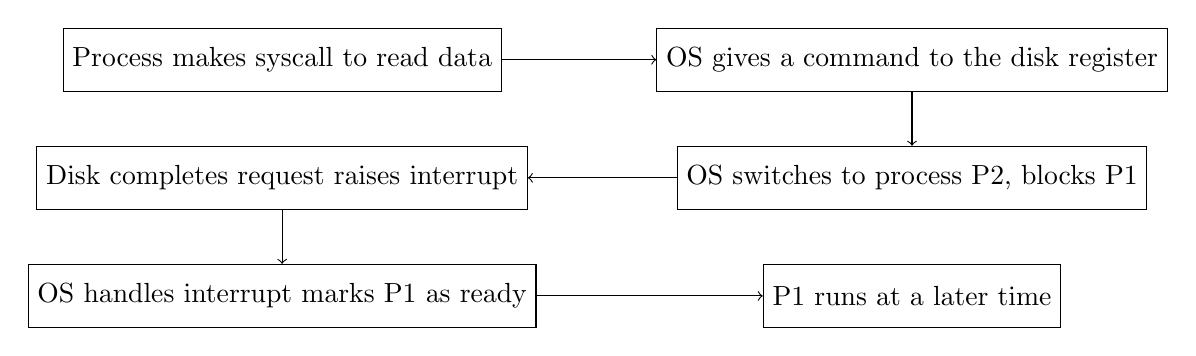
\begin{tikzpicture}[node/.style={rectangle, draw, minimum size=0.8cm}]
    \node[node] (n1) at (0,0) {Process makes syscall to read data};
    \node[node] (n2) at (8,0) {OS gives a command to the disk register};
    \node[node] (n3) at (8,-1.5) {OS switches to process P2, blocks P1};
    \node[node] (n4) at (0,-1.5) {Disk completes request raises interrupt};
    \node[node] (n5) at (0,-3) {OS handles interrupt marks P1 as ready};
    \node[node] (n6) at (8,-3){P1 runs at a later time};


    
    \draw[->] (n1.east) -- (n2.west);
    \draw[->]  (n2.south) -- (n3.north);
    \draw[->]   (n3.west) -- (n4.east);
    \draw[->]   (n4.south) -- (n5.north);
    \draw[->]   (n5.east) -- (n6.west);
    % \draw[->] (n2.east) -- (n3.west);
    % \draw[->] (n3.east) -- (n4.west);
\end{tikzpicture}



\section{File Abstractions}

Some defintions to be known:
\begin{itemize}[topsep = 0cm, parsep = 0cm, itemsep = 0cm]
    \item\textbf{File:} is a sequence of stored persistently/permanently on disk.
    \item \textbf{Directory:} is a container for files and other sub-directories. 
    \item \textbf{File System:} is the OS subsystem that stores all files and directories on a secondary device like a harddisk, provides interface to them via syscalls. It is bulit upon as layers. The syscalls use the generic block interface, which uses the device driver for specific functions to actually communicate with the device.
    \item \textbf{Device Driver:} Part of the OS code that talks to a specific device, gives commands, handles interrupts\ldots etc. Most OS code abstracts out the 
    device-specific details. A device also comes with a device driver code that enales us to communicate with it. 
\end{itemize}

\subsection{Directory Tree}
As seen a directory is a special file that stores the mappings between filenames and something called their \textbf{inode} number. 
It can be visualised as a tree like structure since there is an underlying hierarchy as a dircetory stores other dircetories `beneath it'.
The parent dircetory which is not contained in any other dircetory is usually called the `root'.

A branch of the tree terminates in a non-directory file which cannot contain any other files in it. It can also terminate on an empty directory. 
\begin{figure}[H]
    \centering
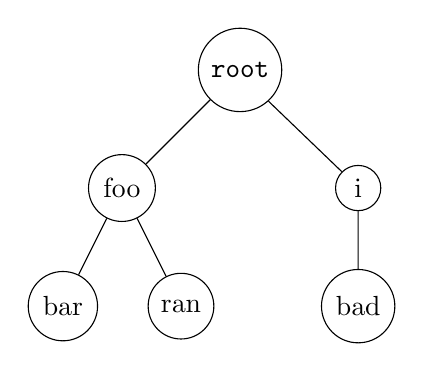
\begin{tikzpicture}[
    every node/.style={circle, draw,minimum size =0.5cm},
    level 1/.style={sibling distance=3cm},
    level 2/.style={sibling distance=1.5cm}
  ]
    \node {\texttt{root}}
      child { node {foo}
        child { node {bar} }
        child { node {ran} }
      }
      child { node {i}
        child { node {bad} }
      };
  \end{tikzpicture}

  \caption{Example of a directory structure}
\end{figure}
Each file has a path from the root. This is called the `path' of a file. It is a represented as a string where the directories on the path are seperated by a /. 
For example the path of bad is ``root/i/bad''.

\subsection{Reading and writing a file}
In order for a process to access a file it needs to be opened by the process. That is the process creates a structure which maintains information about the file and obtaines a pointer to the file. These `file structures' are maintained in an array and the index corresponding to a particular file is called its \textbf{file descriptor}.

Inorder to perform read/write operations on a file we can use syscalls which take its file descriptor as a parameter. The \texttt{read()} syscall reads a particular number of bytes into a user defined buffer a pointer to whom is passed as a parameter. Similarly the \texttt{write()} syscall 
writes a particular number of bytes from a user-define buffer into a file.

Both read and write syscalls alter the \textit{offset} of a file. Initially the offset of a file is set to 0\footnote{For a reading operation} (or) the beginning of a file. As we read the offset gets updated and the next read happens at the (n+1)\(^\text{th}\) byte. This offset can also be updated by the user using the \texttt{seek()} syscall. 
Note that the same file can be opened multiple times by a process and each instance has a different file descriptor, offset etc\dots

\subsection{Directories, Sockets and pipes}
Even opening a socket or a pipe returns a file descriptor. These objects are treated exactly the same as files. Infact almost everything on a system is treated as a file. 
When a process is created by default it has three file descriptors corresponding to the stdin, stdout, stderr streams. All these I/O streams are also exactly treated as files. 

The directory is a special files that maps the filename to its \textit{inode number} as mentioned before. The indode number is used to uniquely identify a file in a disk. The \texttt{ls} command infact just opens the current directory file and displays all of its contents.

\section{File system}

How are these files organised on a disk?
The disk offers us blocks\footnote{512 bytes size usually} of memory that can be used. The files are organised in these blocks according to the file system. Metadata data are stored in various data structures in these blocks. The system calls extract or insert data into the appropriate blocks associated with a file.
There are two types of blocks, Inode blocks and data blocks
\subsection{Inode Node}
Files are variable sized but are broken into some number of the blocks offered by the disk and stored non continguosly. This is very similar to paging done by the OS. 


How are the blocks associated with a file known? Each file has a block allocated to store metadata about it. This block in which an inode is stored is called the Inode block. All permissions, file size, last access time...etc are stored on the Inode. Most importantly the 
Inode has a certain number of bytes to store pointers to the blocks which contain the actual data of the file itself. These blocks which store data are the data blocks. 


The first set of blocks of the disk is allocated to store inodes of the files present on the disk. Thus there is a restriction on the number of the files that can be stores on the disk.


\end{document}

